%%% Local Variables:
%%% mode: latex
%%% TeX-master: t
%%% End:

\newcommand\xkk[1]{x_{(#1)}}

\subsection{convex domain}
\begin{frame}
  \frametitle{Convex Domain}
\only<1>{
\textbullet Linear Regression method is applicable only if nonlinear function is
linear in terms of function parameters:
$$\dis f(x; a) = \sum_{k=1}^m a_kh_k(x)$$

\textbullet Many nonlinear functions are not like that, for example:
\begin{equation*}
  \begin{split}
f_1(x) & = \frac{x^2}{a_1 + (x - a_2)}\\
f_2(x, y, z) & = \frac{x^2}{a_1 + x^2} + \frac{y^2}{a_2 + y^2} + \frac{z^2}{a_3 + z^2}
  \end{split}
\end{equation*}
}

\only<2>{

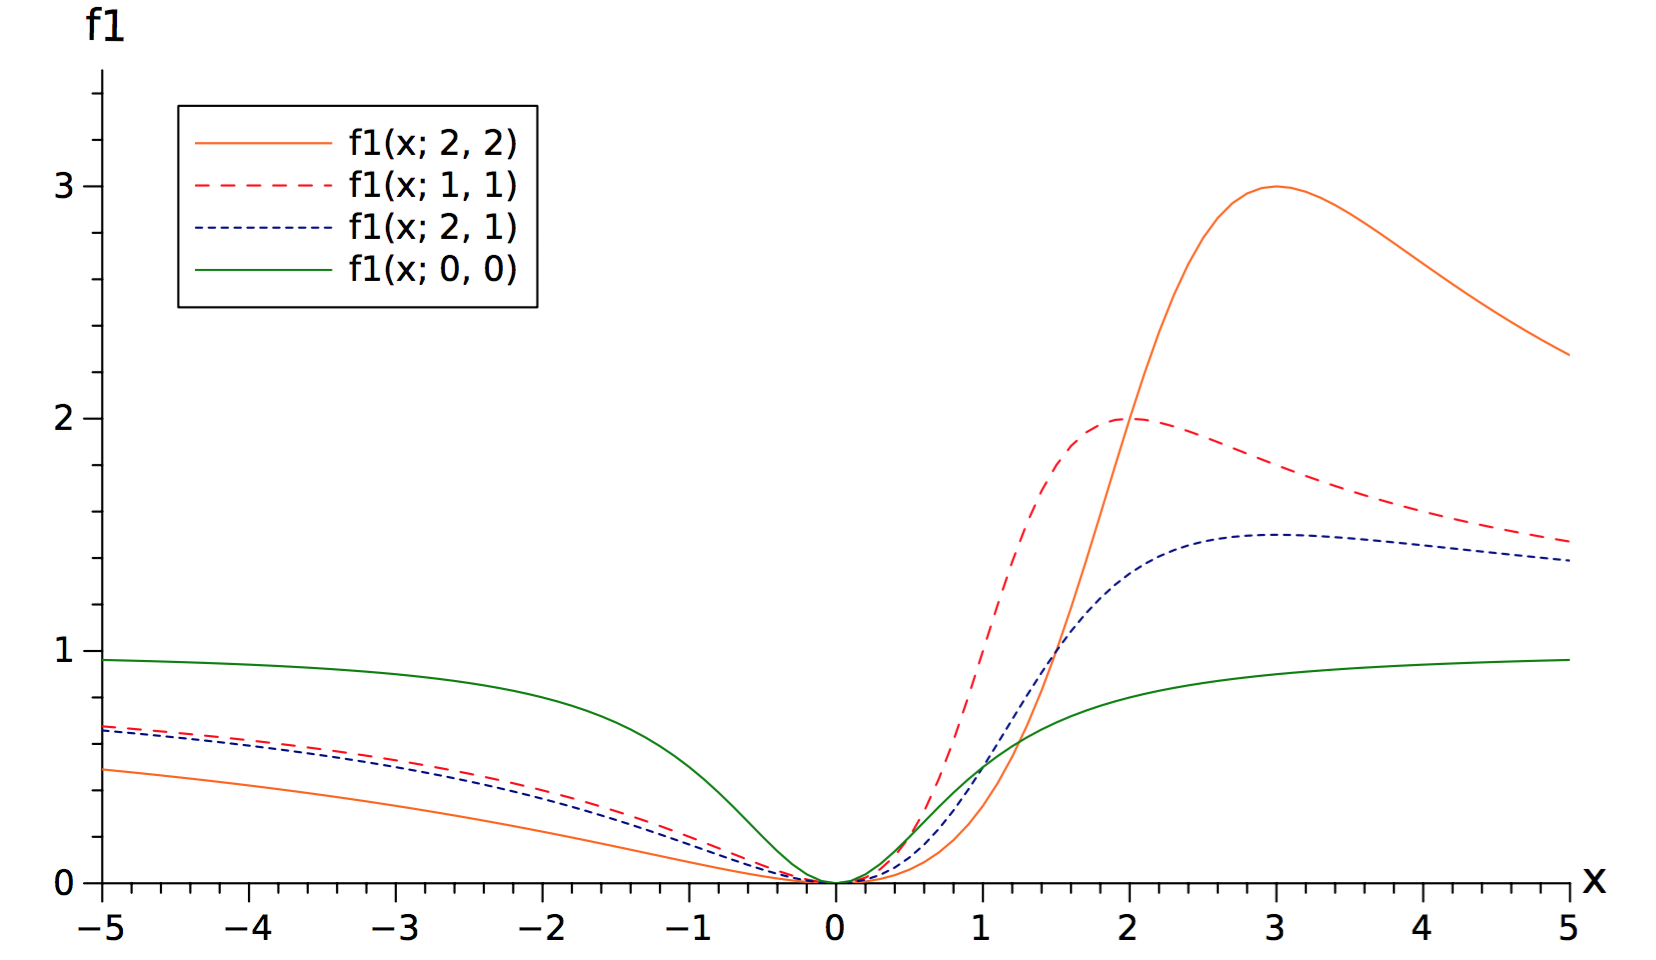
\includegraphics[scale=0.32]{pics/funcs.png}

To minimize the error, we need iterative optimization.
}
\end{frame}


\subsection{limitations}
\begin{frame}
\frametitle{Advantages -- Disadvantages -- Limitations}


\only<1>{
\textbullet If step length is appropriate, $f$ always decreases: converge. {\bf (well
condition)}

\begin{figure}[t]
  \centering
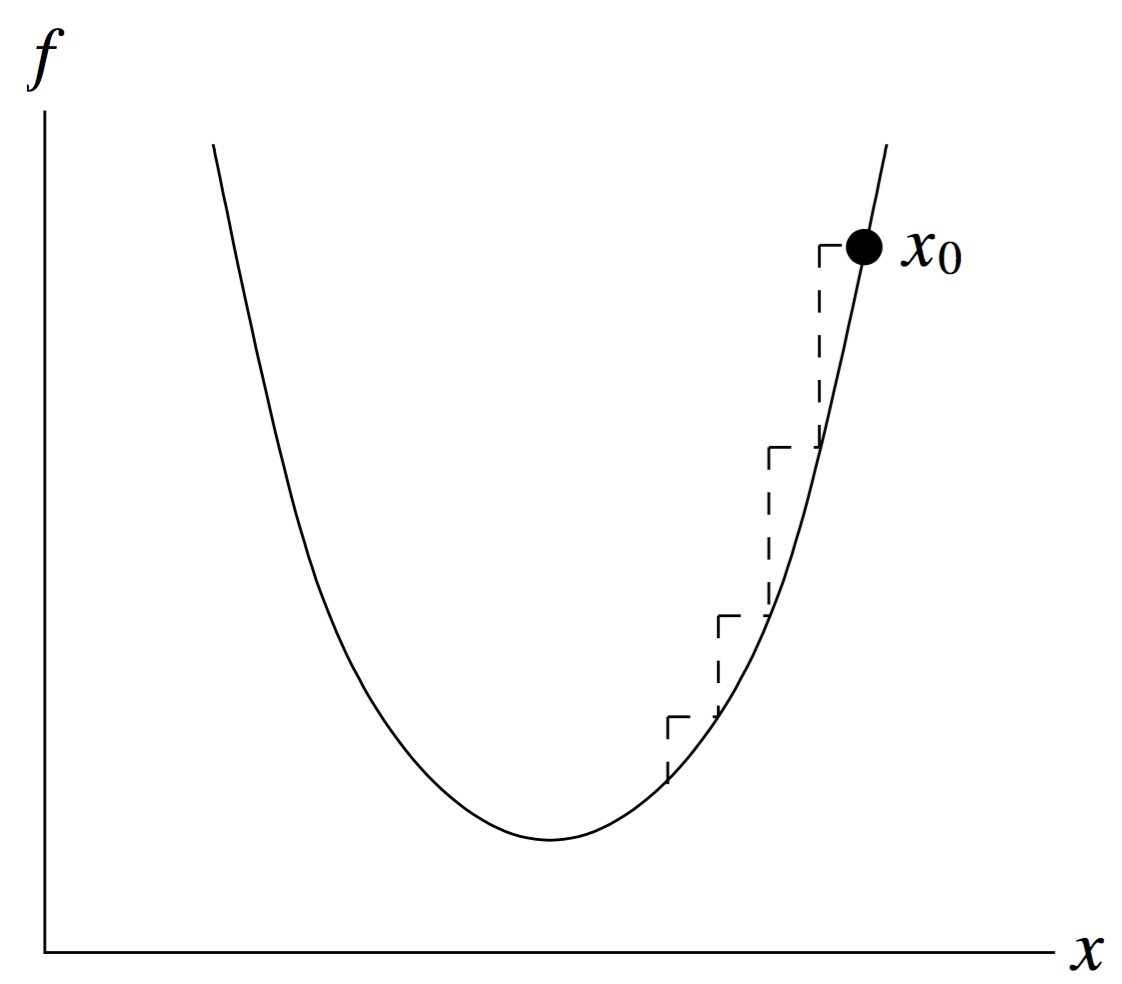
\includegraphics[scale=0.32]{pics/sa.png}
  \caption{Well Conditioned}
\end{figure}


}

\only<2>{
\textbullet If step length is too large, $f$ can increase: diverge. {\bf (ill
  condition)}

\begin{figure}[t]
\centering
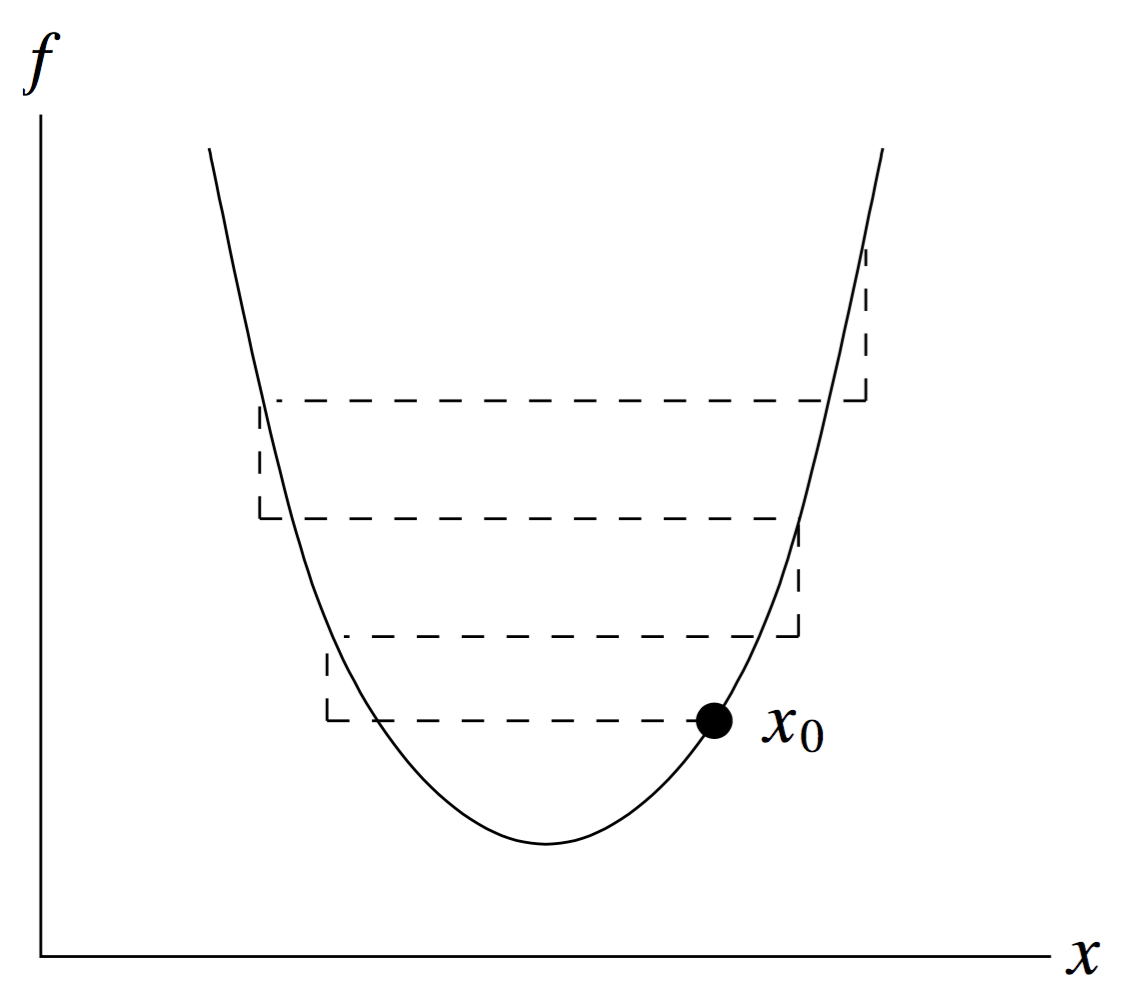
\includegraphics[scale=0.32]{pics/si.png}
\caption{Ill Conditioned.}
\end{figure}


}

\only<3>{
\textbullet If parameters of f affect error equally,

\begin{figure}[t]
\centering
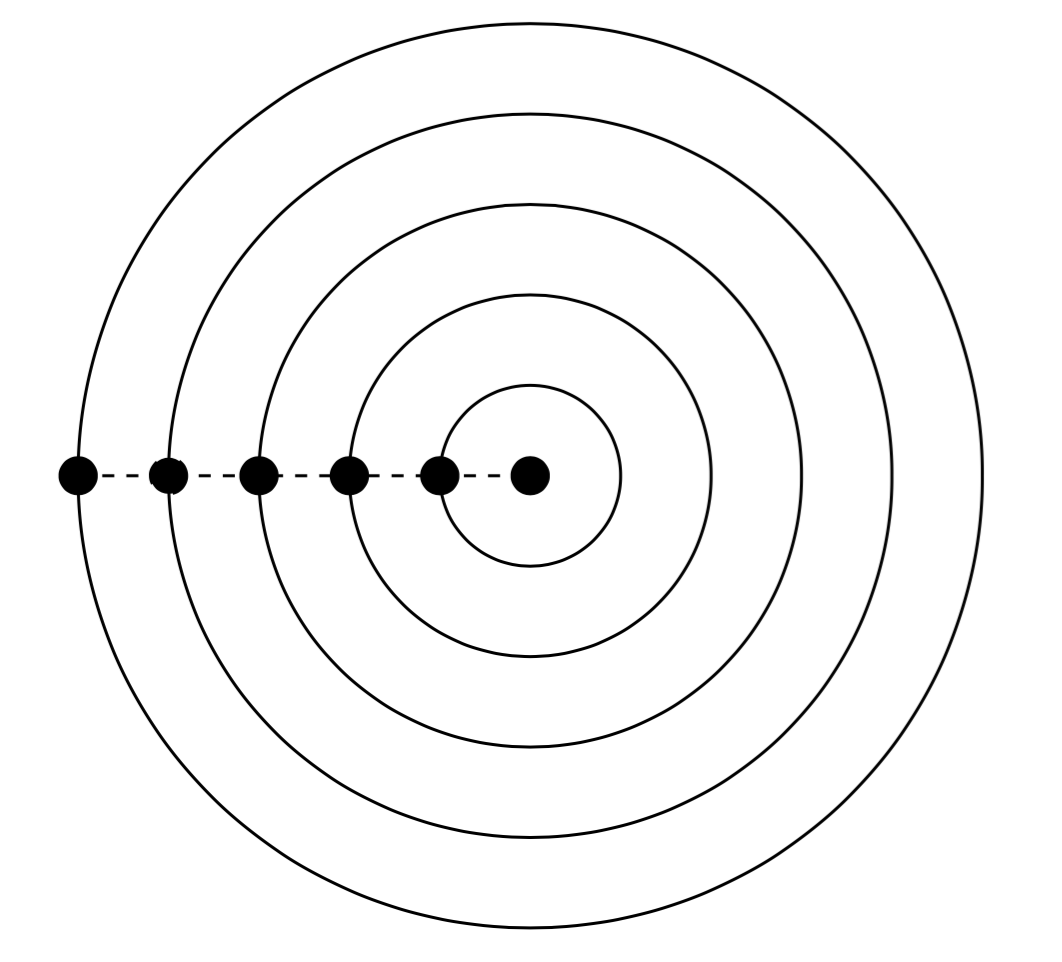
\includegraphics[scale=0.32]{pics/topview.png}
\caption{Straight path, fast convergence. {\bf (well condition)}}
\end{figure}


}


\only<4>{
\textbullet If parameters of f affect error unequally,
\begin{figure}[t]
  \centering
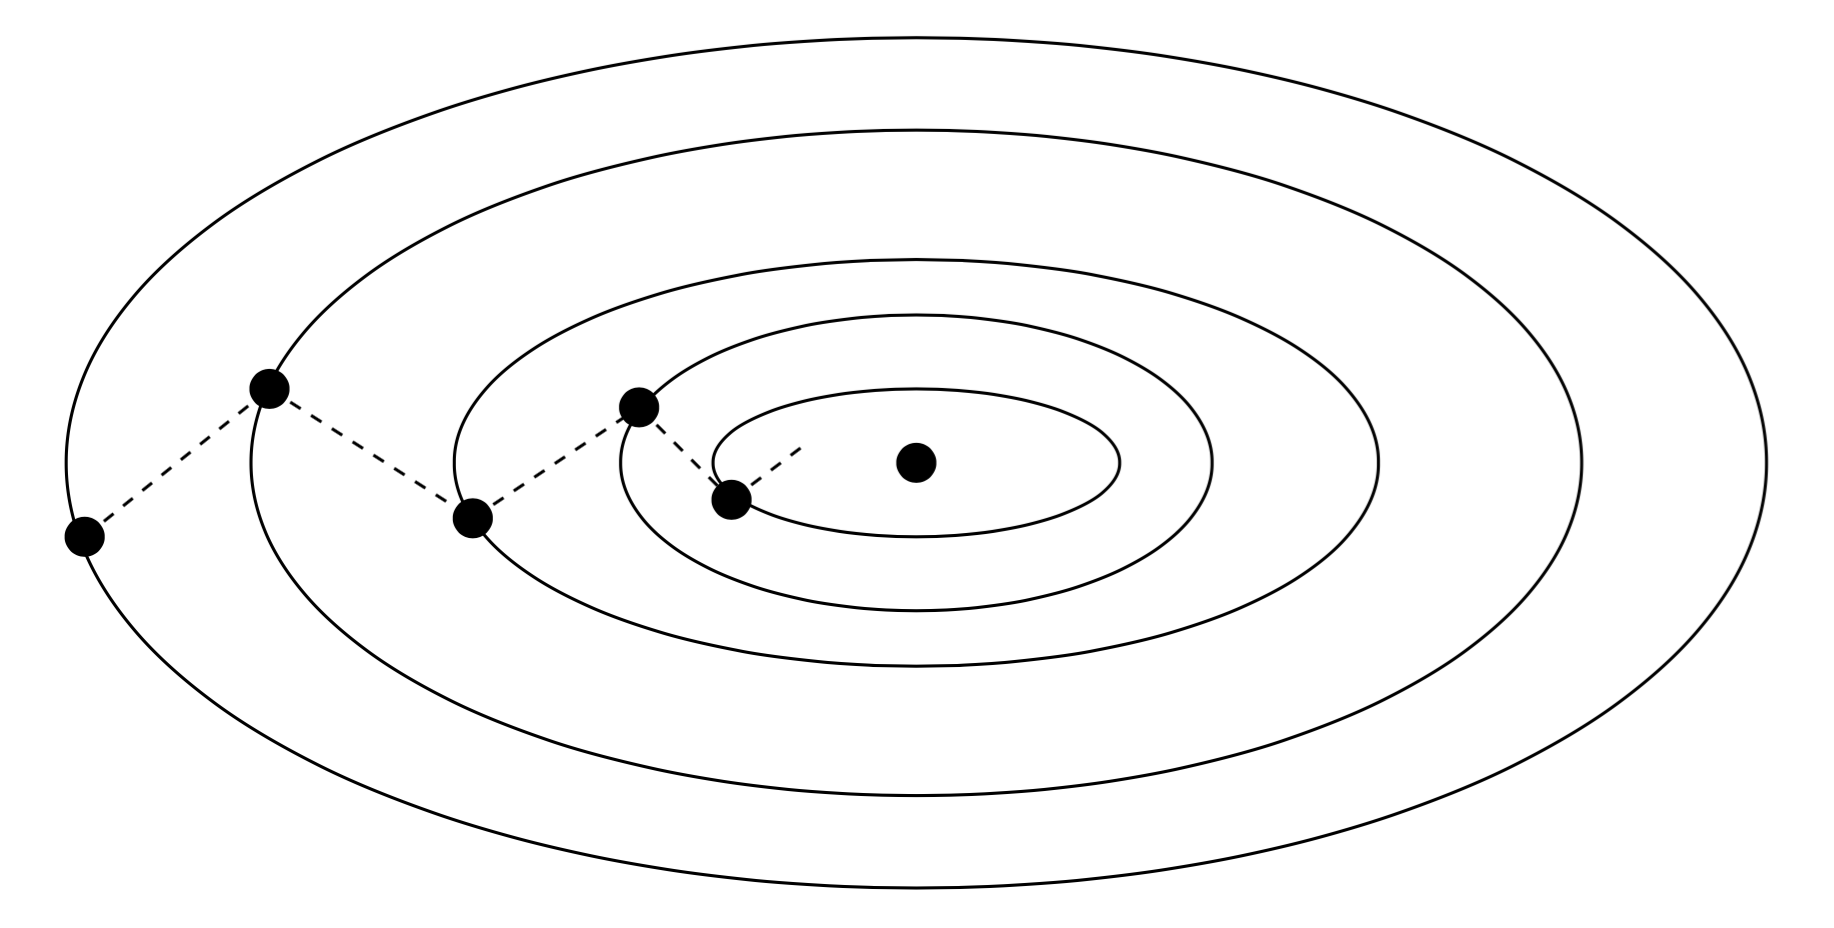
\includegraphics[scale=0.28]{pics/topview2.png}
\caption{Jagged path, slow convergence. {\bf (ill condition)}}
\end{figure}



}


\only<5>{
\textbullet If parameters of f affect error very unequally,

\begin{figure}[t]
  \centering
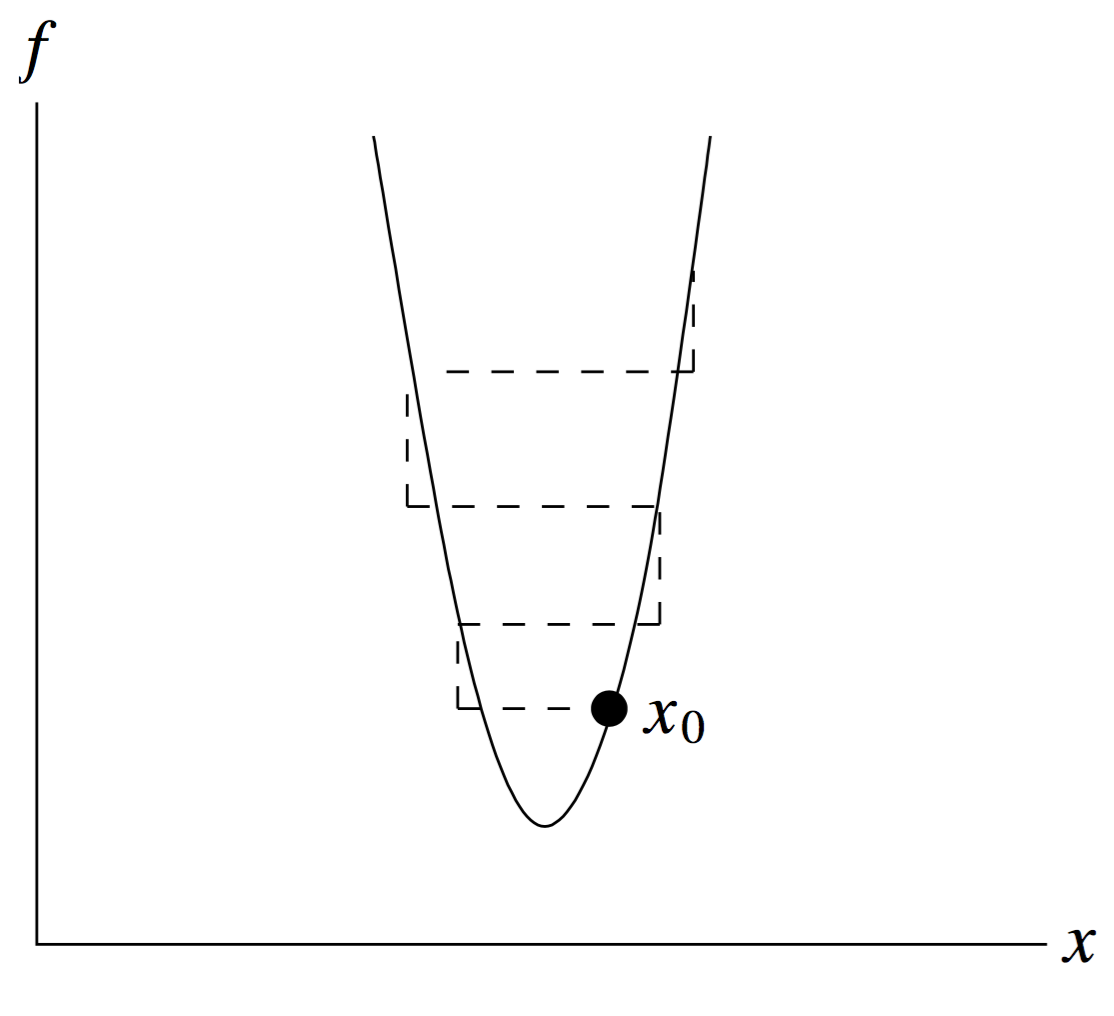
\includegraphics[scale=0.32]{pics/unequal.png}
  \caption{Small step length can also cause divergence. {\bf (ill
      condition)}}
\end{figure}
}

\end{frame}


\begin{frame}
\frametitle{Condition Number}
\begin{itemize}
\item The condition number of C gives a measure of its anisotropy or
  eccentricity.
\item If the condition number of a set C is small (say, near one) it
  means that the set has approximately the same width in all
  directions, i.e., it is nearly spherical.
\item If the condition number is large, it means that the set is far
  wider in some directions than in others.
\item $cond(f) = \frac{\lambda_{max}(f)}{\lambda_{min}(f)}$
\item $\lambda_{max}$ and $\lambda_{min}$ describes minimum and maximum eigenvalues in 2D.
\end{itemize}

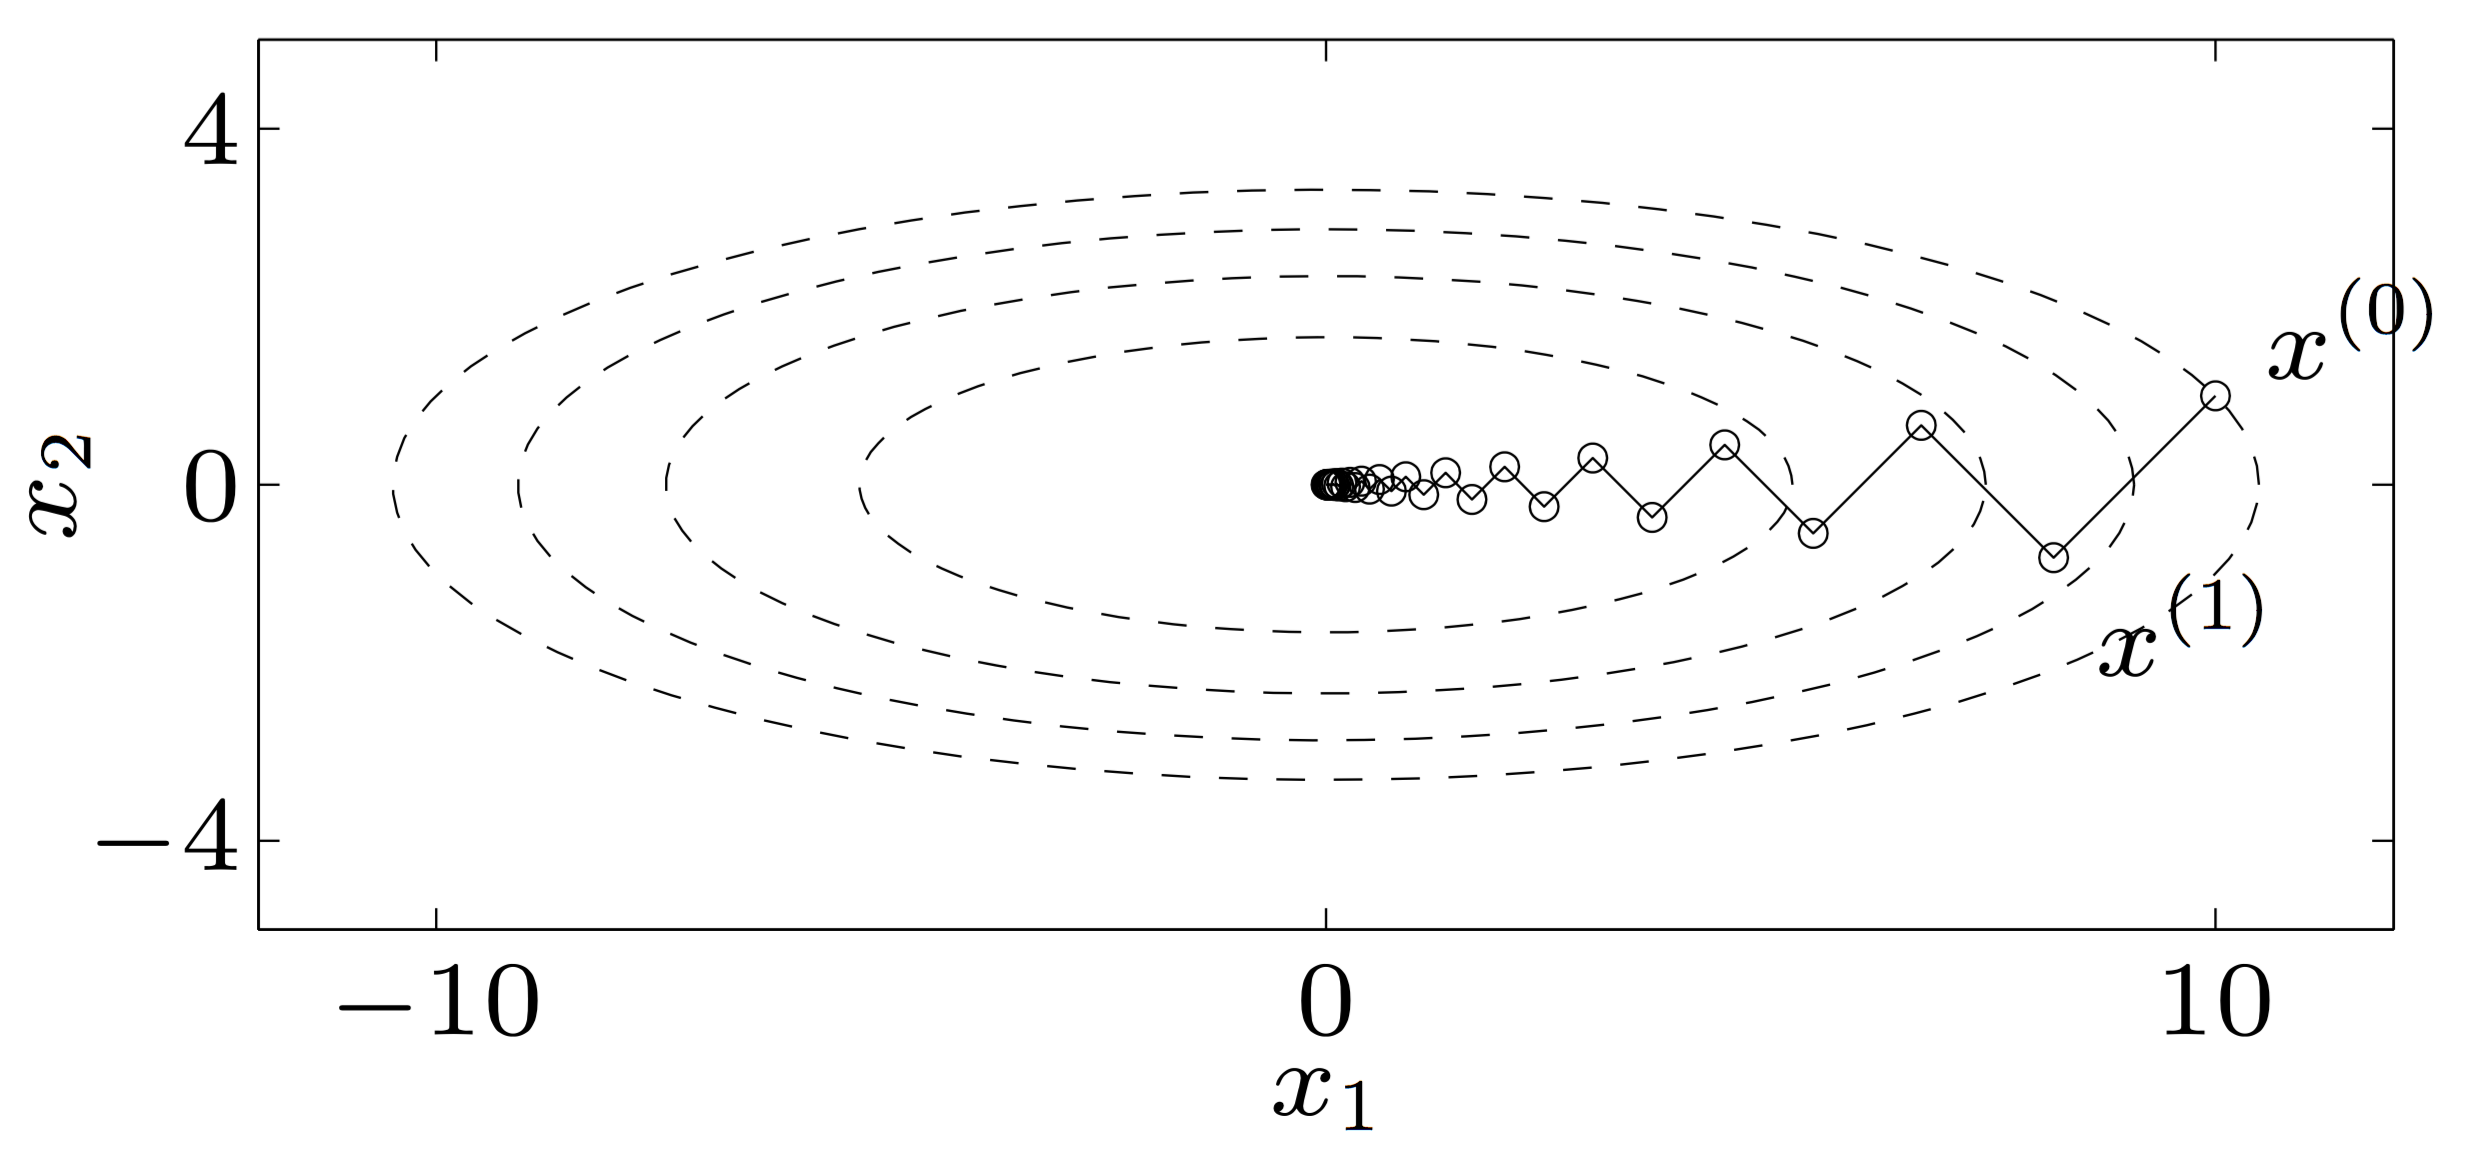
\includegraphics[scale=0.08, right]{pics/example.png}
\end{frame}

\begin{frame}
  \frametitle{Example Quadratic Problem in $R^2$}

{
\tiny

$$f(x) = \frac{1}{2}(x_1^2 + \gamma \xkk{2}^2) ~~~ \gamma > 0$$

with exact line search, starting at $x^{(0)} = (\gamma, 1)$
$$\xkk{1}^{(k)} = \gamma (\frac{\gamma - 1}{\gamma + 1})^k, ~~
\xkk{2}^{(k)} = \gamma (-\frac{\gamma - 1}{\gamma + 1})^k$$
}
\vspace{-8mm}

{
\tiny
\begin{itemize}
\item Hessian of f has eigenvalues 1 and $\gamma$. And, m = $\min\{1,
    \gamma\}$,and $M = \max\{1, \gamma\}$
\item In particular,$f(\xkk{k})$ converges to $p^*$, optimal value, at
  least as fast as a geometric series with an exponent that depends
  (at least in part) on the condition number bound $\frac{M}{m}$.

\end{itemize}


}
\begin{columns}

  \begin{column}{0.6\textwidth}


\begin{itemize}
\item Very slow if $\gamma > 1 or \gamma < 1$
\item Useless if $\gamma > 20$.
\item Example for $\gamma = 10$.
\end{itemize}
\end{column}

\begin{column}{0.5\textwidth}
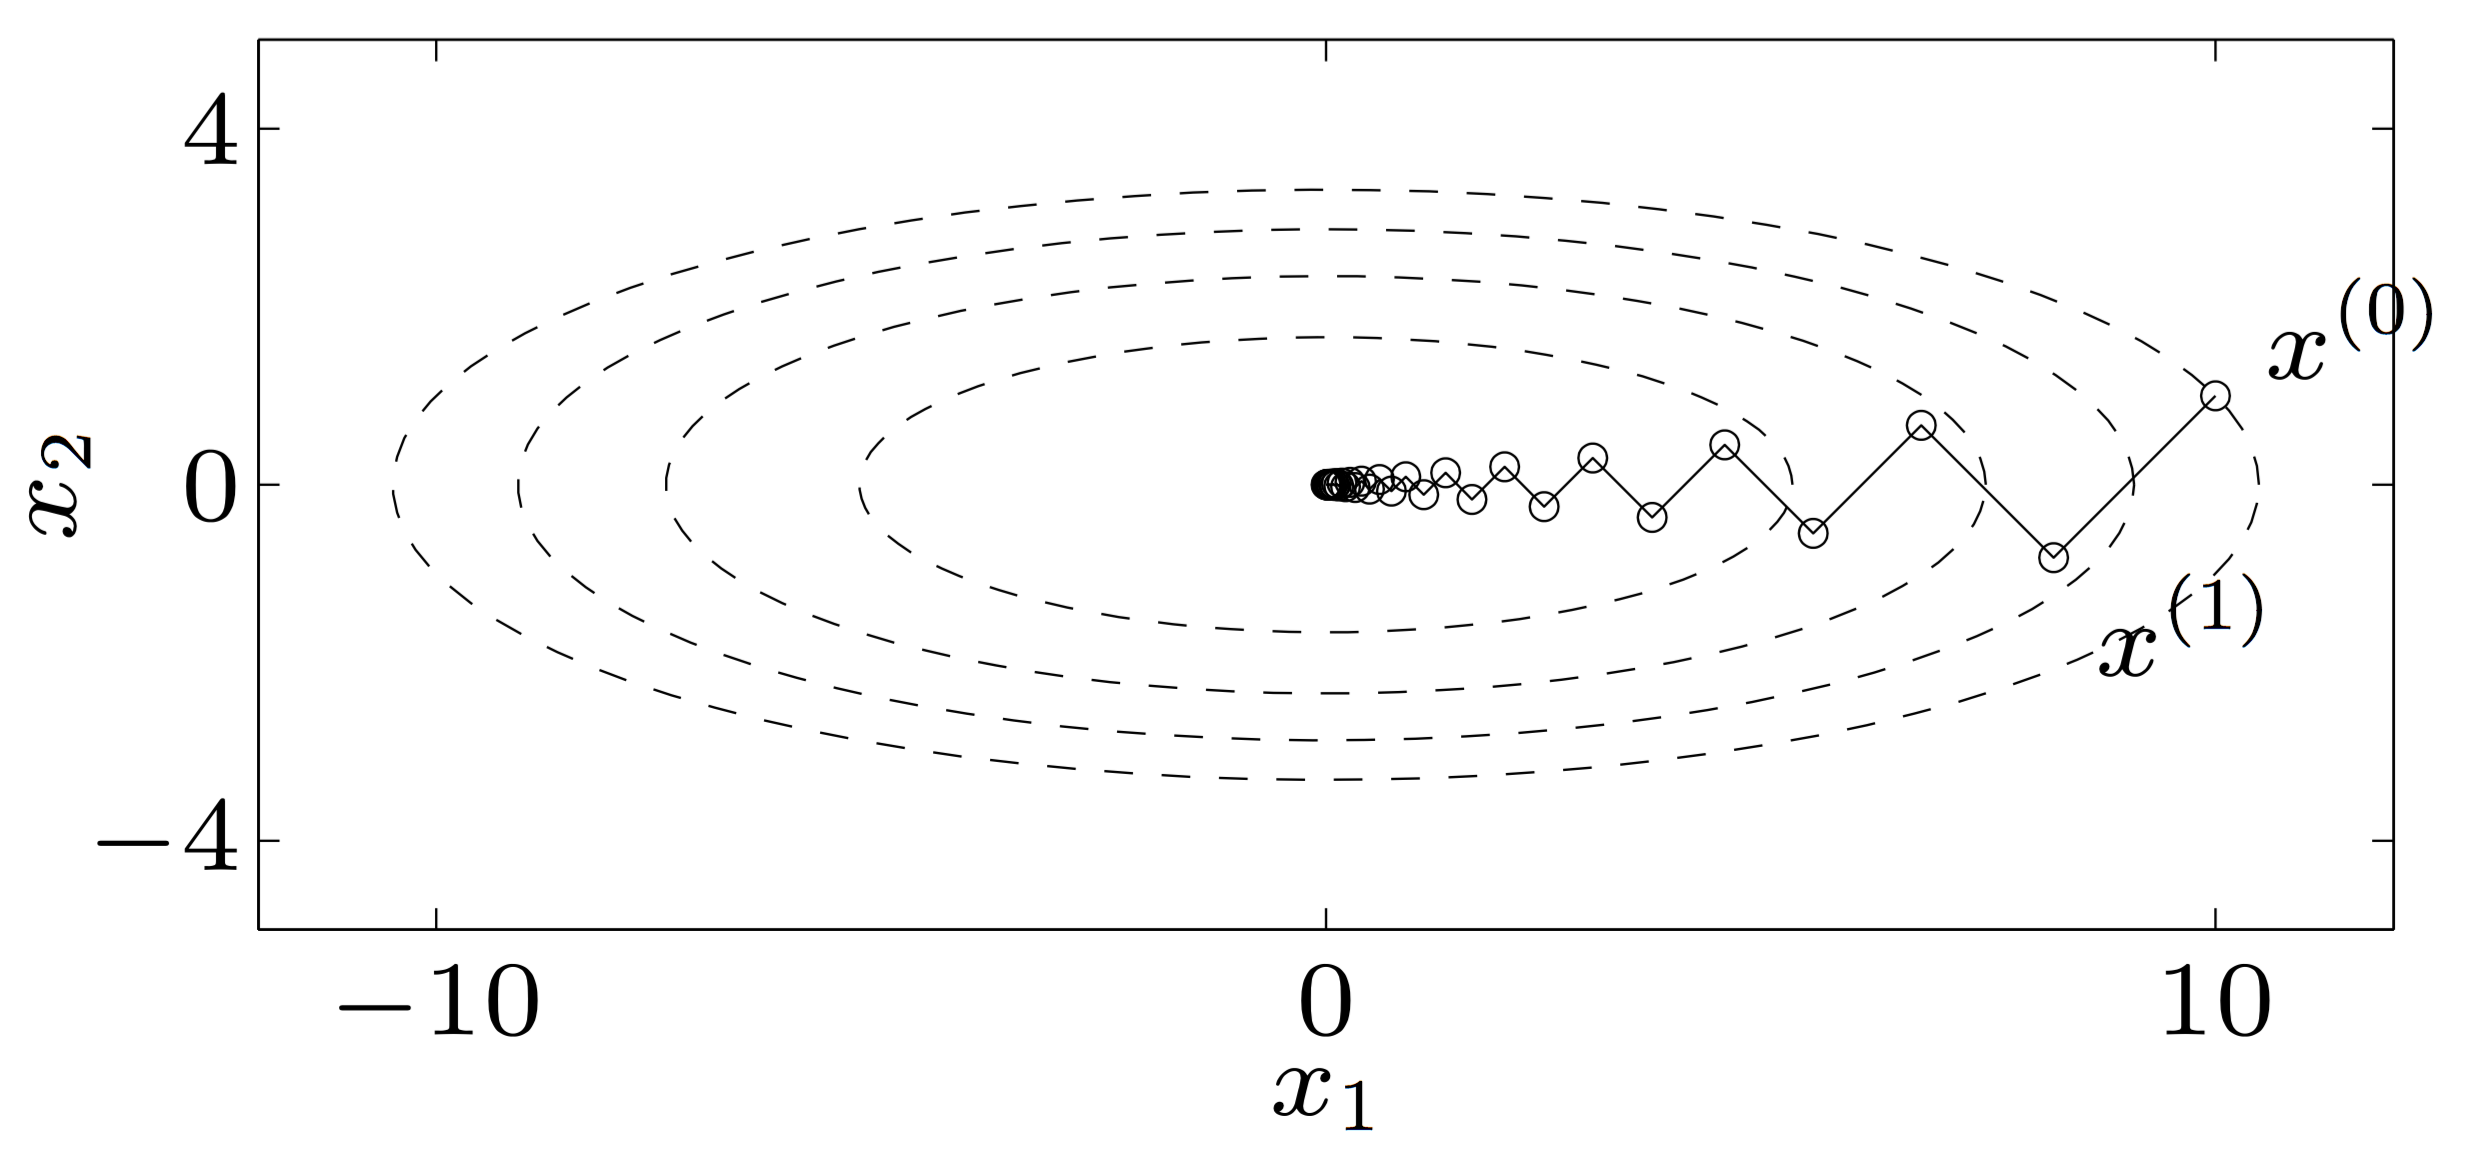
\includegraphics[scale=0.12, center]{pics/example.png}
\end{column}


\end{columns}
\end{frame}


\begin{frame}
  \frametitle{Advantages -- Disadvantages -- Limitations}

  \textbullet { \scriptsize   {\bf\it Left} Number of iterations of the gradient method as a
    function of $\gamma$ which can be thought of as amount of diagonal
    scaling.}

  \textbullet{\scriptsize {\bf\it Right} Condition number of the Hessian of the function at its
    minimum as a function of $\gamma$.}

\textbullet{\scriptsize We see that the condition number has a very strong influence on
convergence rate.}

\begin{columns}
  \begin{column}{0.5\textwidth}
    \begin{figure}[ht!]
      \centering
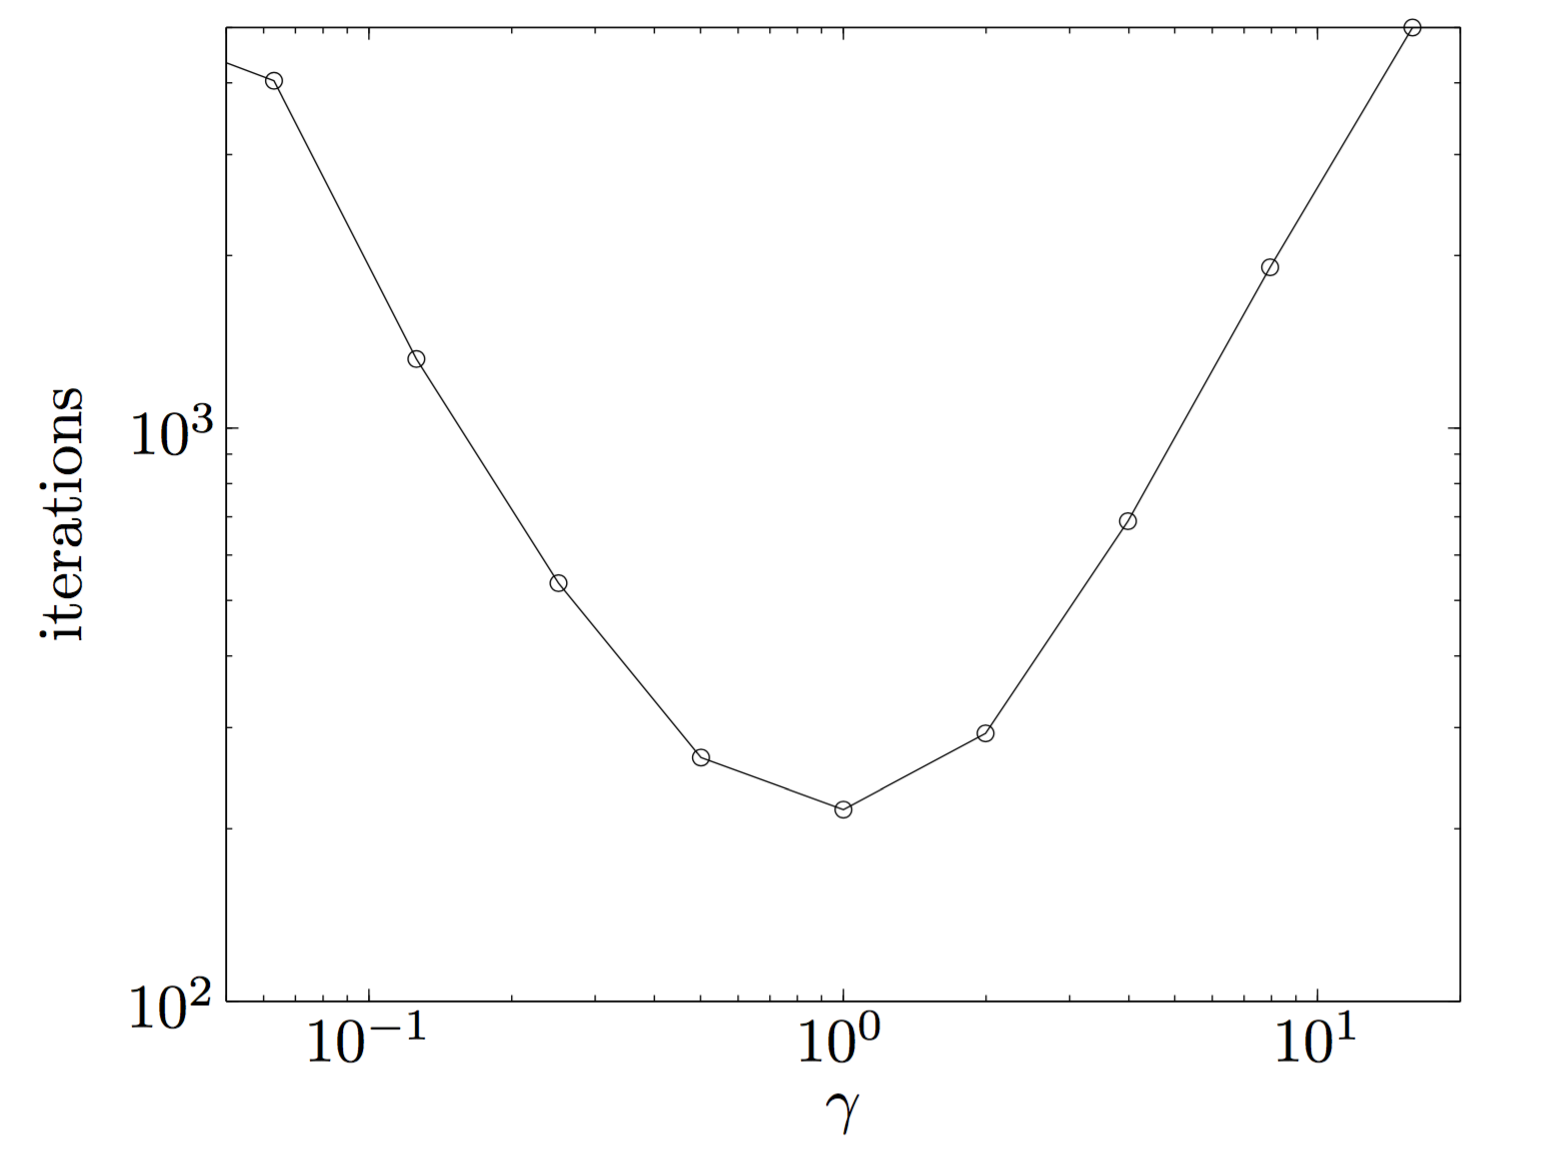
\includegraphics[scale=0.15]{pics/ga1.png}
\caption{\tiny The
  verticle axis shows the number of iterations required to obtain
  $\overline{f}(\overline{x}^{(k)}) - \overline{p}^* < 10^{-5}$. The
  horizontal axis shows $\gamma$, which is the  parameter that controls the amount of diagonal scaling. We use a
backtracking line search with $\alpha = 0.3, \beta = 0.7$.}
    \end{figure}
  \end{column}

  \begin{column}{0.5\textwidth}
    \begin{figure}[ht!]
      \centering
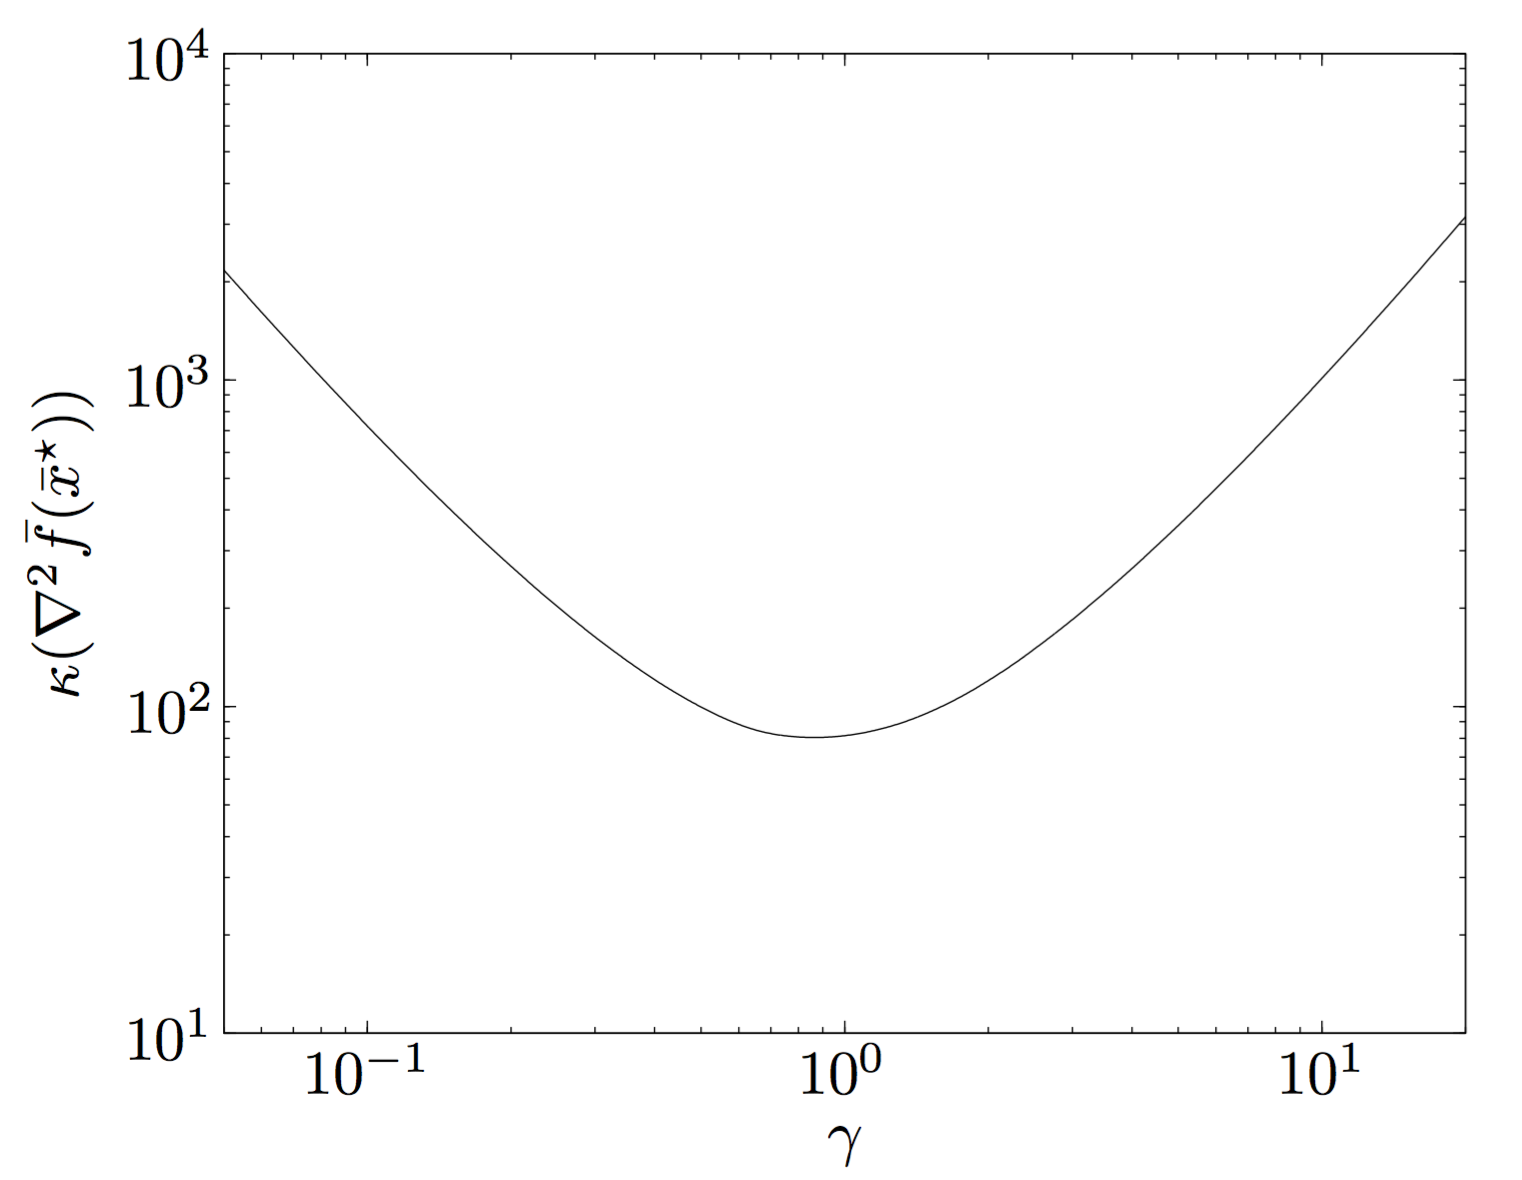
\includegraphics[scale=0.15]{pics/ga2.png}
\caption{\tiny Condition number of the Hessian of the function at its
  minimum, as a function of $\gamma$. By comparing this plot with the
  one in the left figure, we see that the condition number has a very strong influence on convergence rate.}
    \end{figure}
  \end{column}
\end{columns}
\end{frame}

\begin{frame}
  \frametitle{Exact Line Search VS.  Backtracking Line Search with
    Non-Quadratic Example}
$$f(x_1, x_2) = e^{x_1+3x_2-0.1} + e^{x_1-3x_2-0.1} + e^{-x_1-0.1}$$

\begin{figure}
\centering
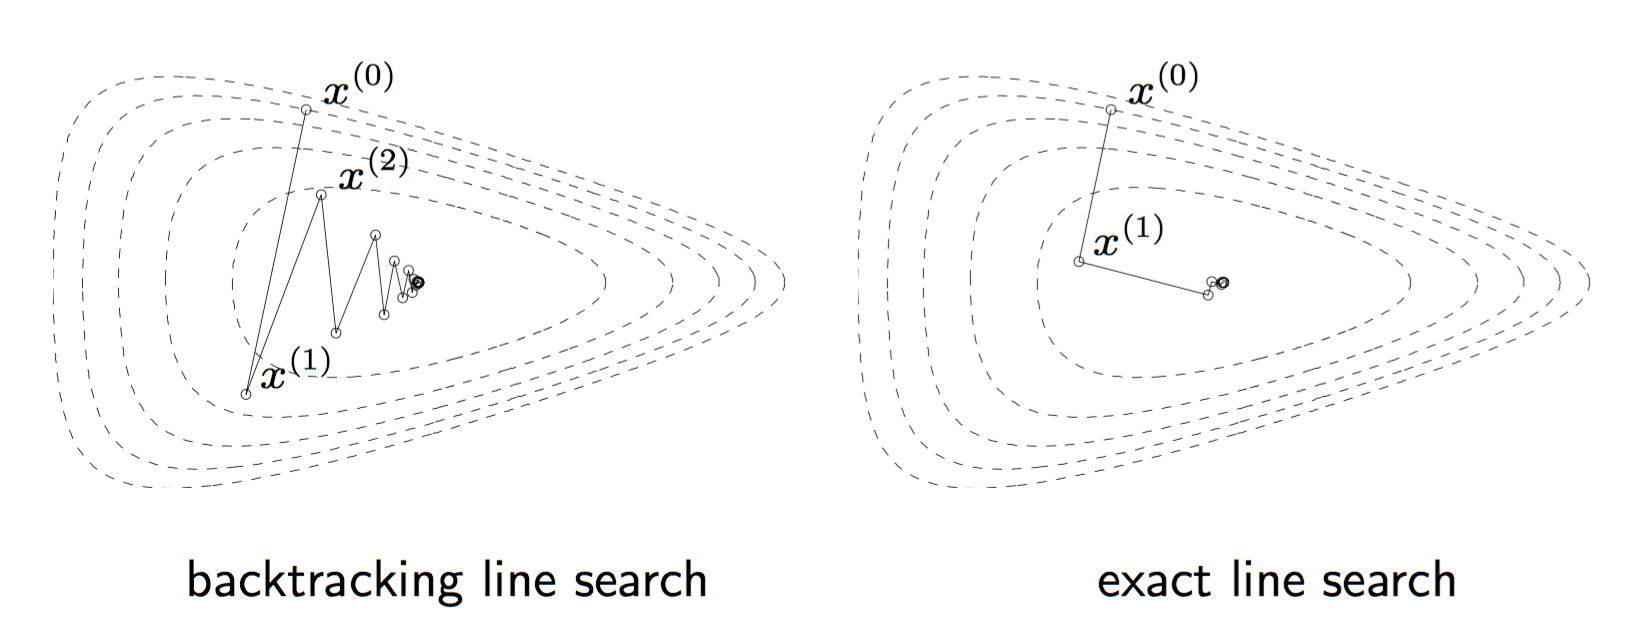
\includegraphics[scale=0.25]{pics/btes.png}
\end{figure}



\begin{columns}
  \begin{column}{0.6\textwidth}
{\tiny
    \begin{itemize}
    \item With exact line search, the error is reduced about $10^{-8}$
      in 20 iterations, i.e., a reduction by a factor of
20 about $10^{-\frac{8}{20}} \approx 0.4$ per iteration.
\item With backtracking line search, the error is reduced
about $10^{-11}$ in 15 iterations, i.e., a reduction by a factor of
15 about $10^{-\frac{11}{15}} \approx 0.2$ per iteration.
    \end{itemize}
}
  \end{column}

\begin{column}{0.5\textwidth}
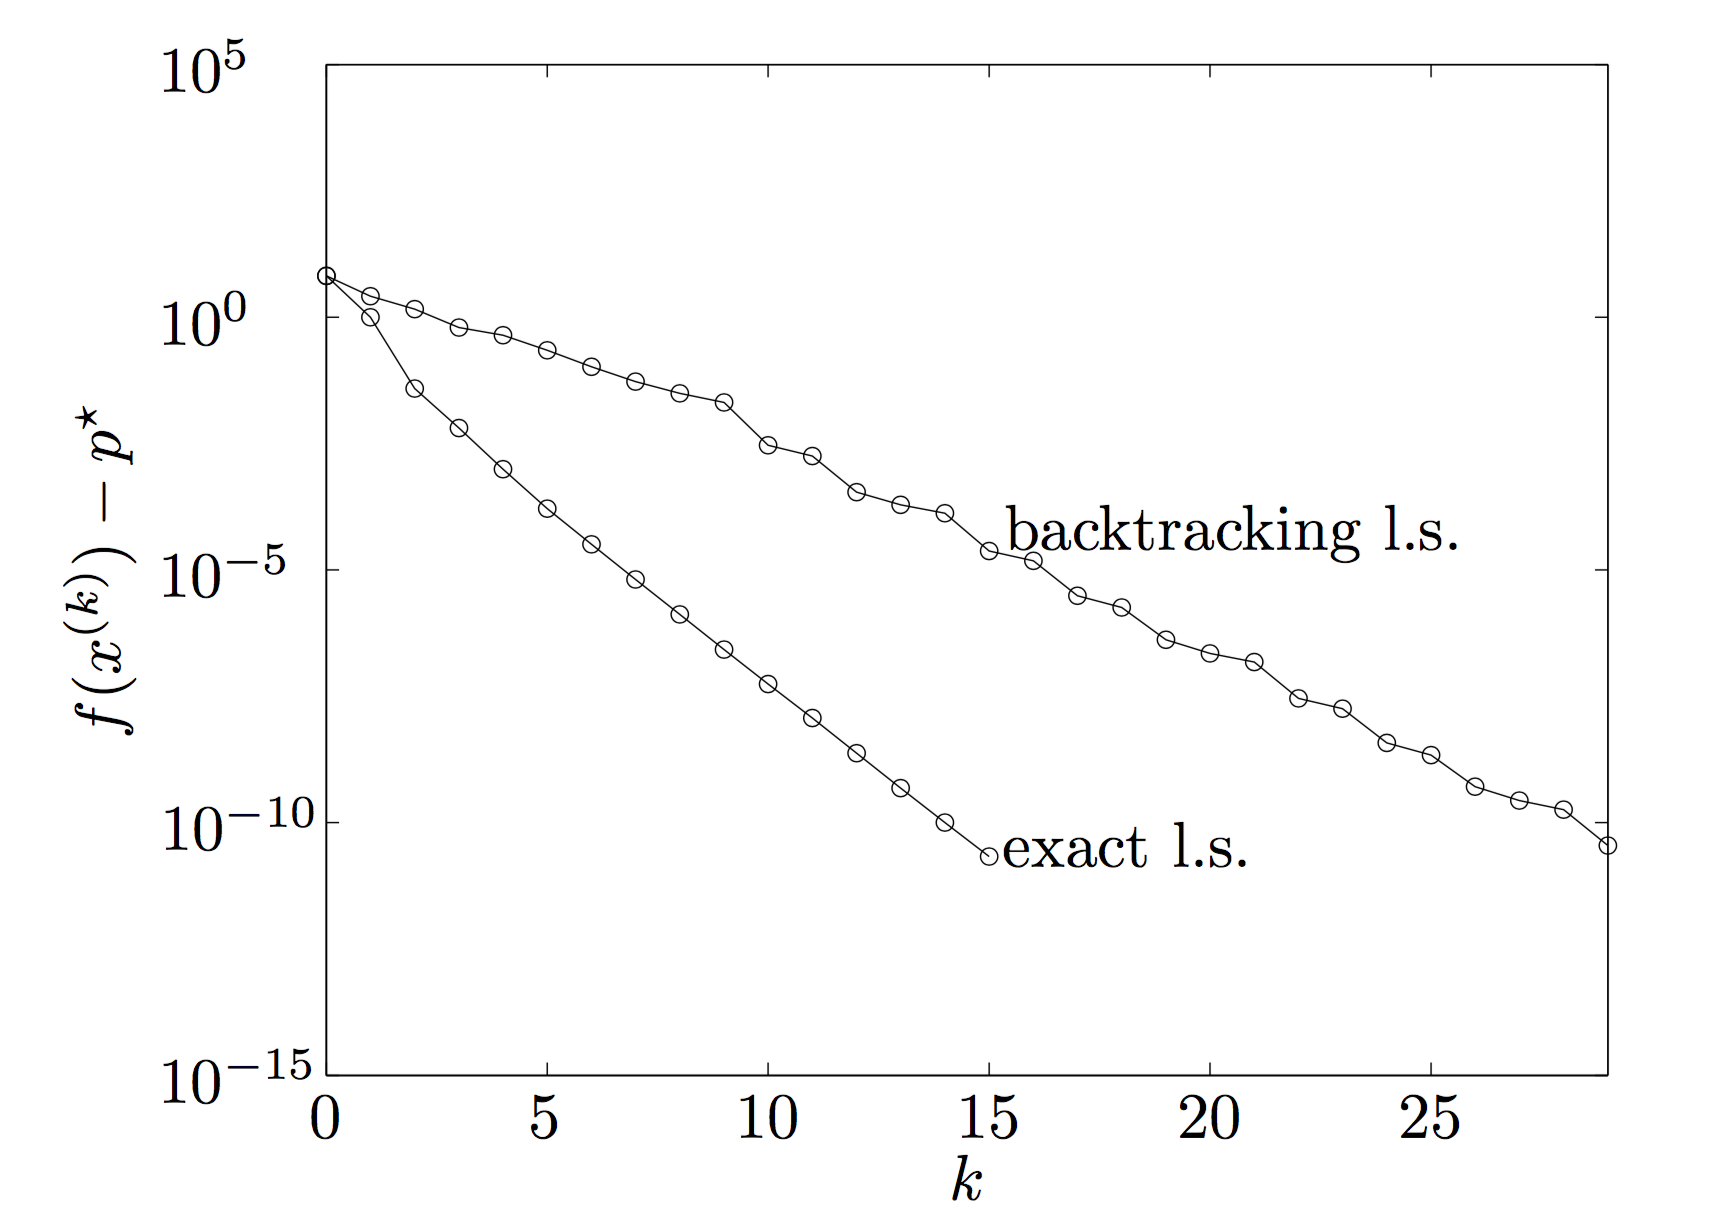
\includegraphics[scale = 0.12]{pics/els.png}

\end{column}

\end{columns}
\end{frame}


\begin{frame}
  \frametitle{Exact Line Search VS.  Backtracking Line Search with
    a Problem in $R^{100}$}

\only<1>{

$$f(x) = c^Tx - \sum_{i=1}^{500}\log(b_i - a_i^Tx)$$
A larger example, of the form with $m = 500$ terms and $n=100$
variables.

\begin{figure}[t]
  \centering
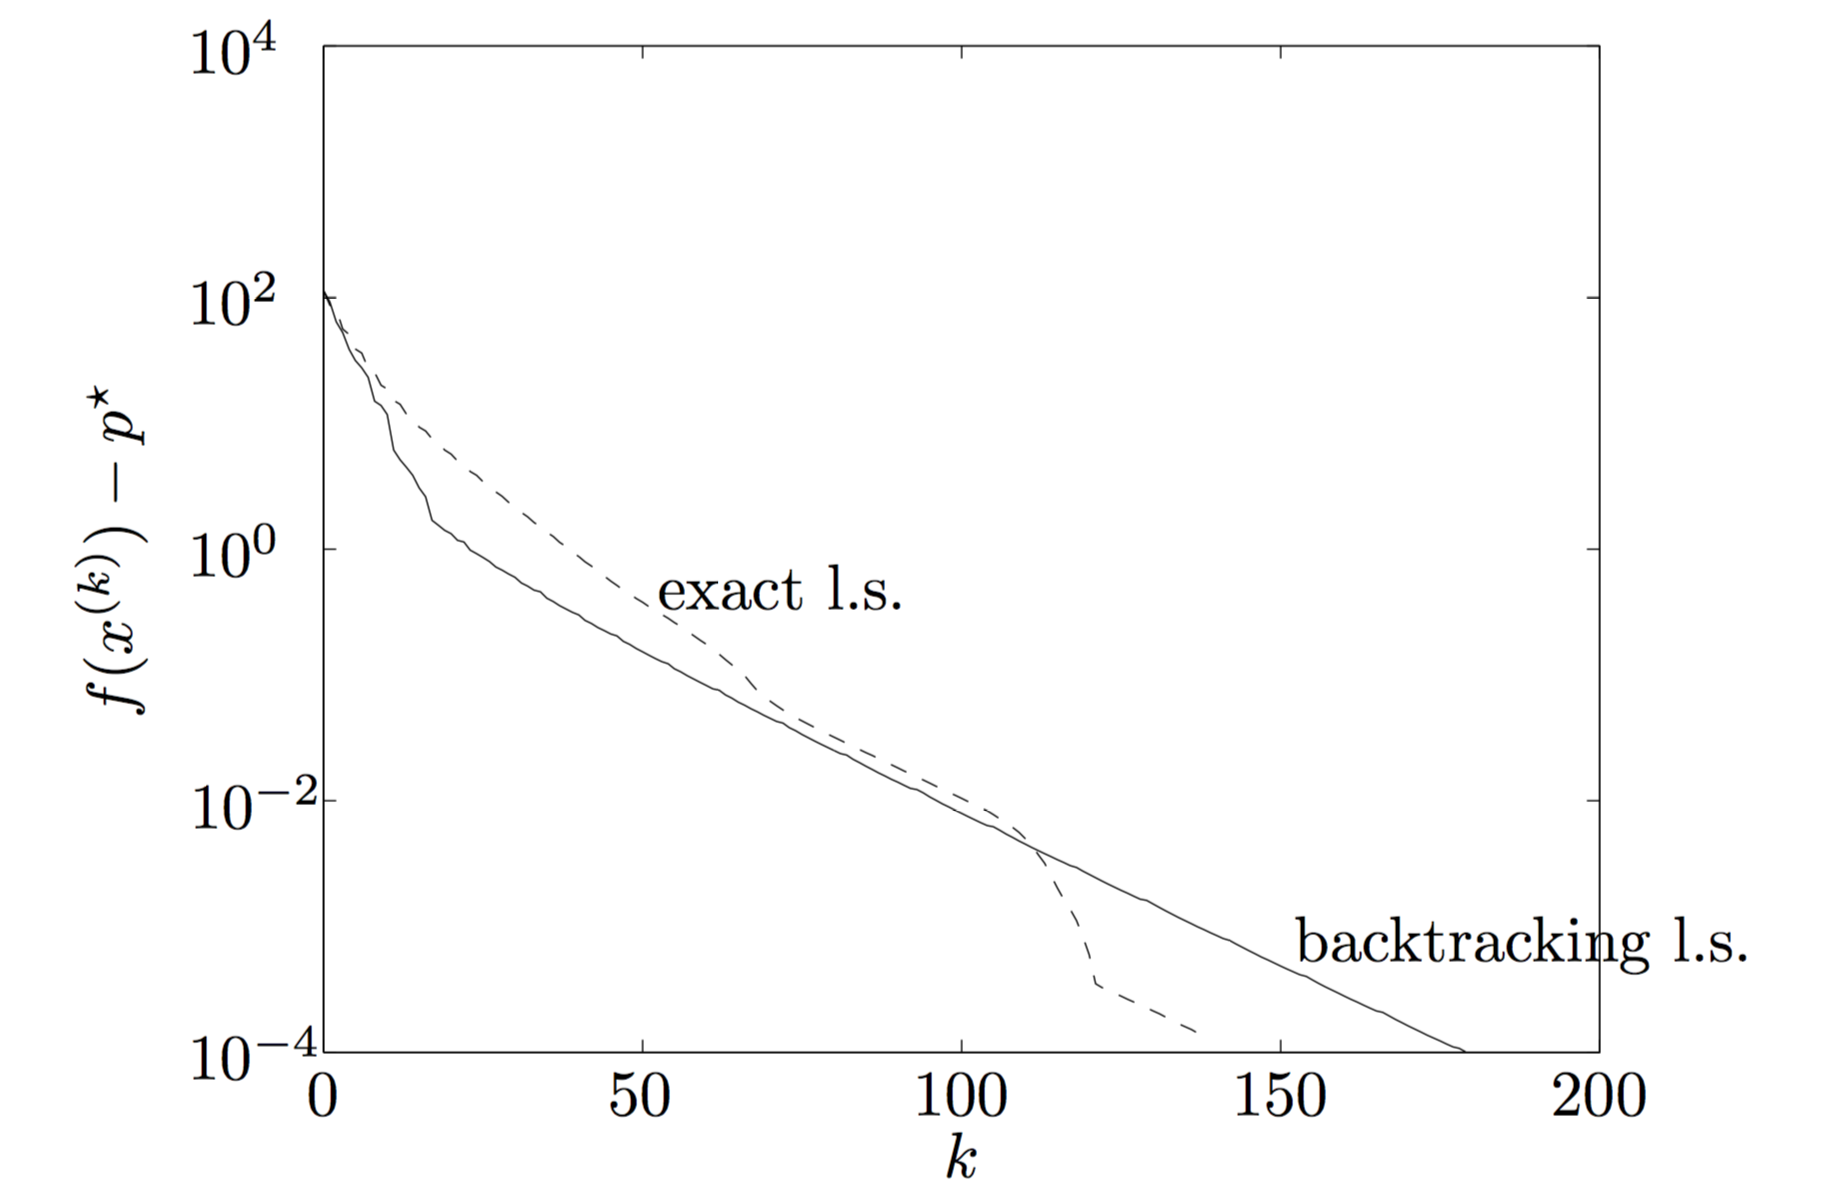
\includegraphics[scale = 0.2]{pics/error.png}
\caption{\tiny ‘linear’ convergence, i.e., a straight line on a semilog plot}
\end{figure}


}

\only<2>{
\textbullet The progress of the gradient method with backtracking line search,
with parameters $\alpha = 0.1, \beta = 0.5$.

\textbullet {\bf Average error reduction} is $10^{-\frac{6}{175}} \approx 0.92$
per iteration.

\begin{columns}
  \begin{column}{0.6\textwidth }
\textbullet In the convergence of the gradient method with exact line search,
{\bf average error reduction} is $10^{-\frac{6}{140}} \approx 0.91$ per iteration. A bit
faster than the gradient method with backtracking line search.
  \end{column}

  \begin{column}{0.5\textwidth}

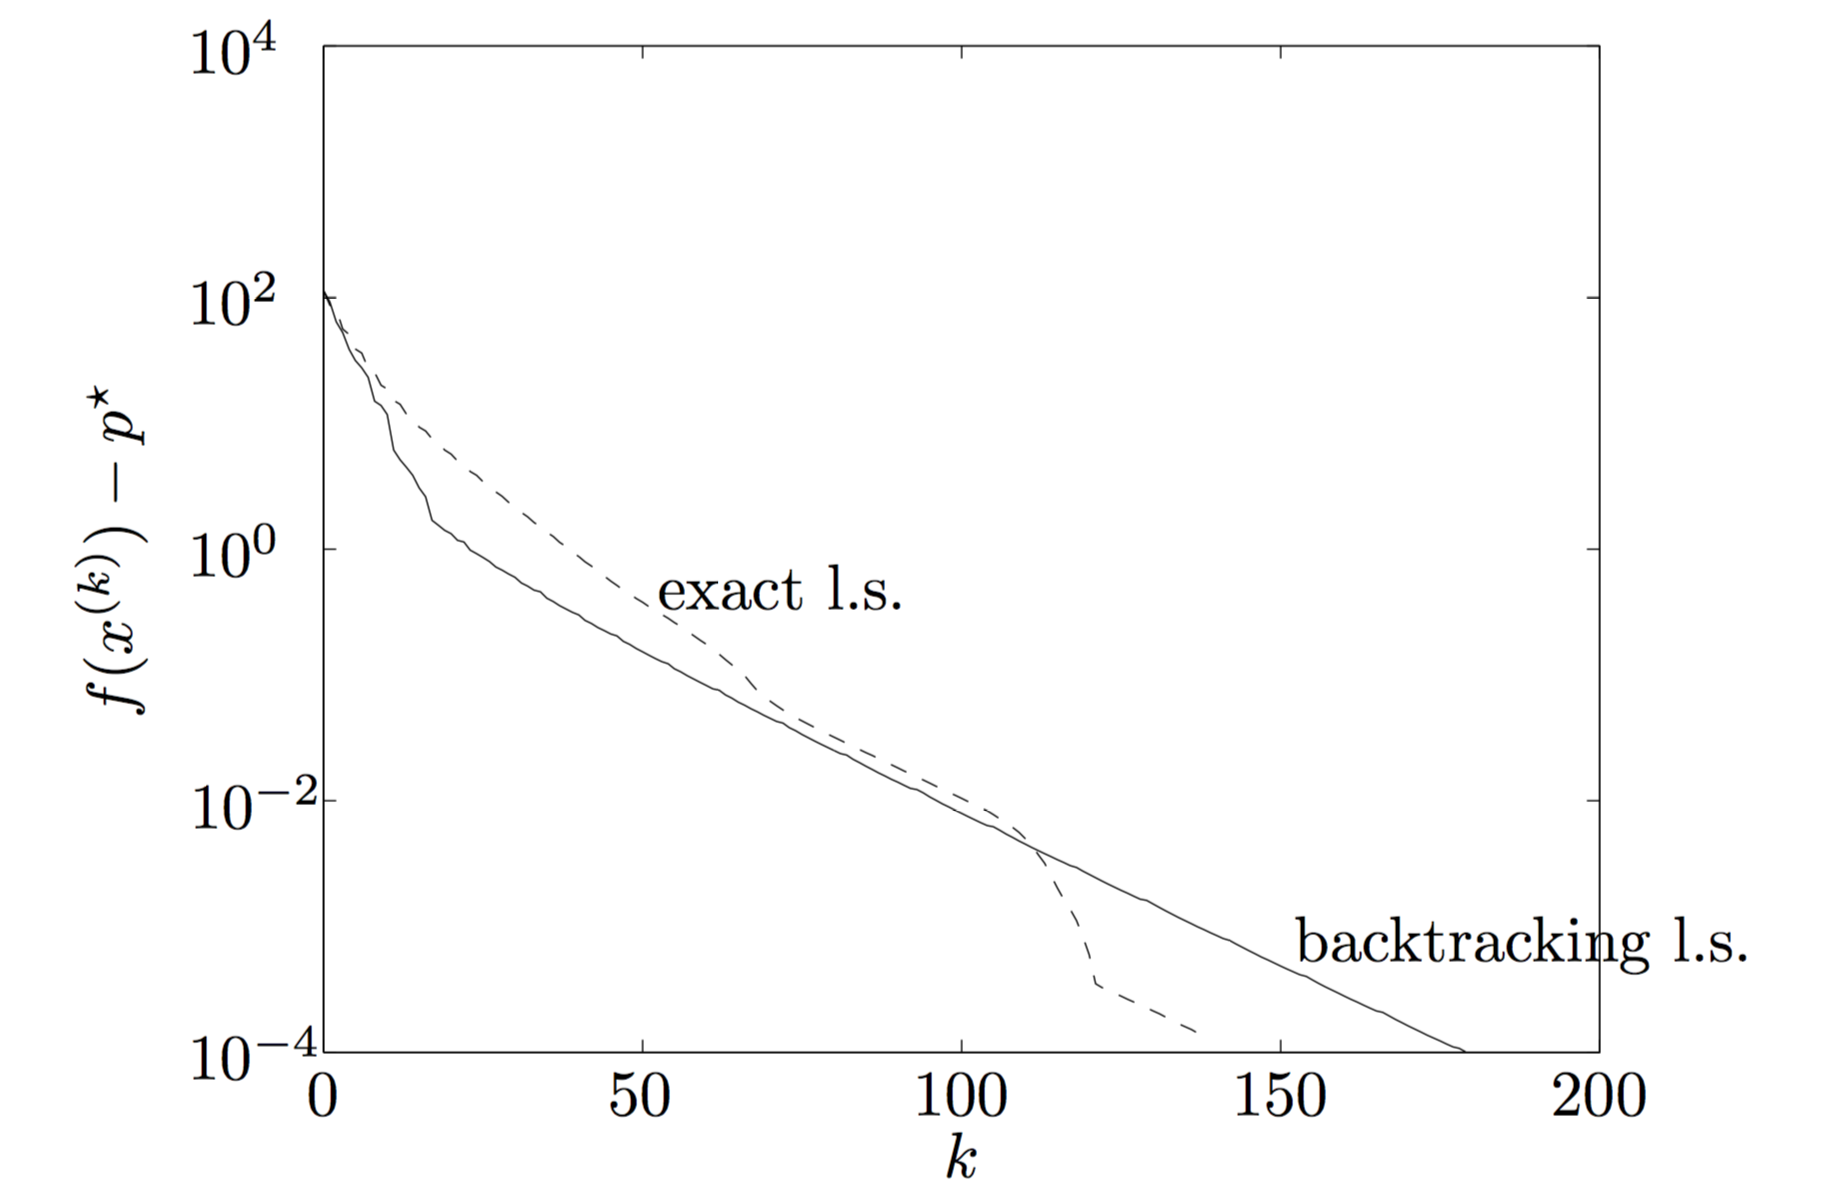
\includegraphics[scale = 0.15]{pics/error.png}
  \end{column}
\end{columns}

}

\only<3>{

  \textbullet These experiments, done by the book authors, show that the
  effect of the {\bf backtracking parameters} on the convergence is
  {\bf not large}.

 \textbullet {\bf Experiment 1}: (effect of the choice of $\alpha$): Fix
  $\beta = 0.5$, and vary $\alpha$. This experiment suggests that the
  gradient method works better with fairly large $\alpha$, in the
  range $(0.2, 0.5)$.

 \textbullet {\bf Experiment 2}: (effect of the choice of  $\beta$): Fix
  $\alpha = 0.1$, and vary $\beta$. This experiment suggests that
  $\beta \approx 0.5$ is a good choice.



}

\end{frame}

\subsection{}
\begin{frame}
  \frametitle{Advantages -- Disadvantages -- Limitations (Gradient
    Descent)}
To summarize here:
  \begin{itemize}
  \item The gradient descent often shows linear convergence.,
i.e. error converges to zero as a geometric series.
\item Choice of the two parameters $\alpha, \beta$ (backtracking parameters) has
  a noticeable effect on convergence, but not dramatic.
\item Exact line search sometimes improves the convergence of the
  gradient method, slightly. However implementation is troublesome.
\item Convergence rate depends on the condition number of the Hessian,
  and this is main disadvantage.
\item The main advantage of gradient method is simplicity.
  \end{itemize}

\end{frame}


\begin{frame}
  \frametitle{Advantages -- Disadvantages -- Limitations (Steepest
    Descent)}

\only<1>{
  \begin{itemize}
  \item For steepest descent, choice of norm is critical. When Euclidian norm
is used the algorithm coincides with the gradient descent method.
When $l_1$ norm is chosen, the algorithm is called “Coordinate
Descent”.
\item The idea is to descend along each coordinate direction
  iteratively.

  \end{itemize}

 Let $e_1, ... ,e_m$ denote the unit vectors along coordinates
  $1, ... ,m$.

      \begin{algorithm}[H]
        \small
        Choose initial $x_0$\;
        \Repeat{convergence}{
          {\bf For $i = 1, ... , m$:} \;
          ~~Find $x_{k+1}$ along $e_j$ that minimizes $f(x_k)$. Or find
          $x_{k+1}$ along $e_j$ using line search to reduce $f(x_{k})$ sufficiently.
        }
        % \caption{Descent Method Algorithm}
      \end{algorithm}
}

\only<2>{
Coordinate descent can be slow. It can also iterate around the
minimum, never approaching it.

\begin{figure}[t]
\centering
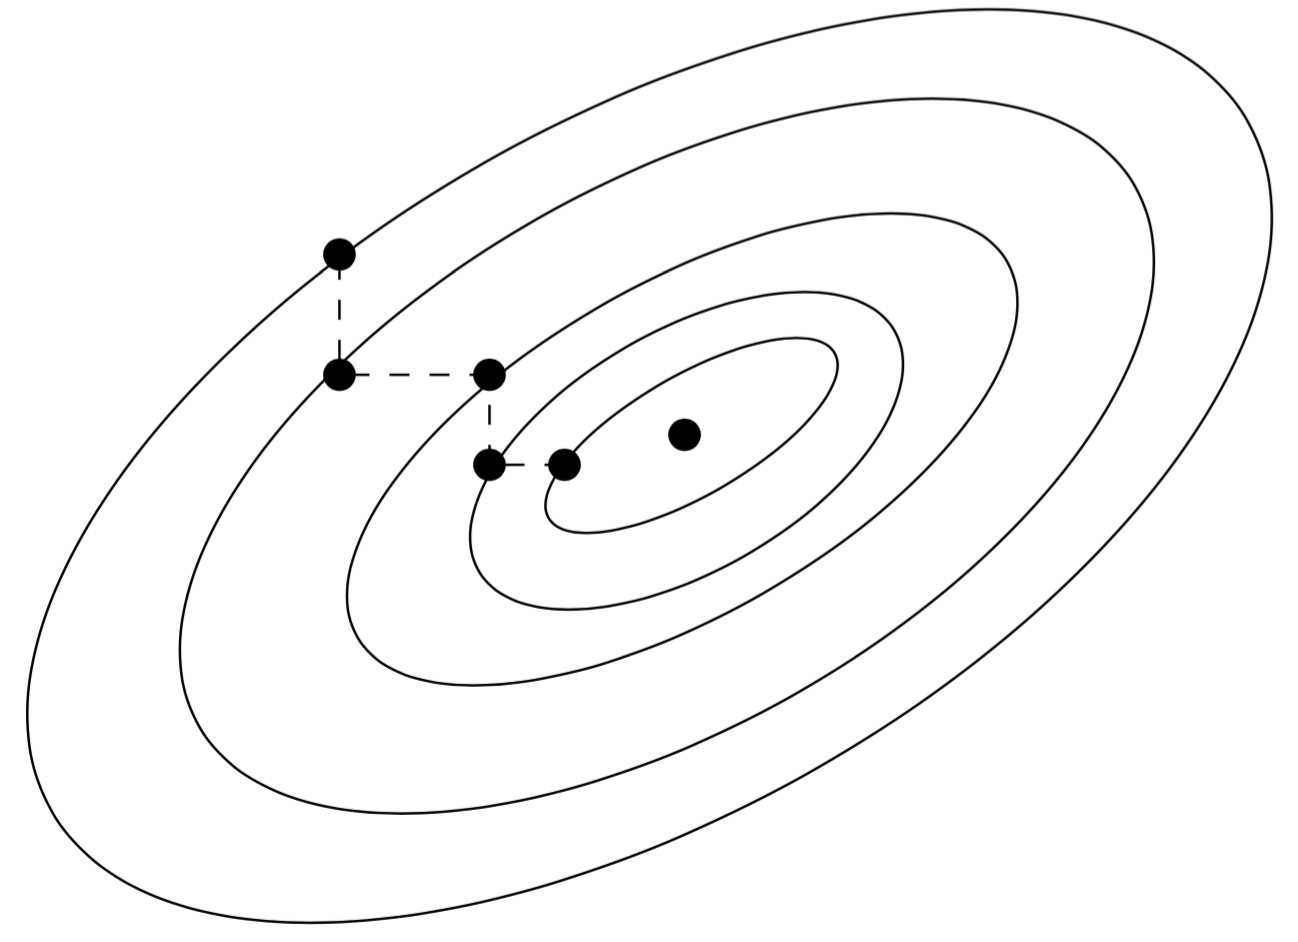
\includegraphics[scale=0.3]{pics/nc.png}

\end{figure}
}

\only<3>{
\textbullet Steepest descent method with the quadratic P-norm $\norm{\cdot}_P$ can
be thought of as the gradient method applied to the problem after the
change of coordinates $\overline{x} = P^{\frac{1}{2}}x$.

\textbullet In the case of steepest descent with {\bf quadratic P-norm}, {\bf
  choice of P} is important.

\textbullet For example: $P = \bigl(\begin{smallmatrix}
2&0 \\ 0&8
\end{smallmatrix} \bigr)$
Choice of $P$ helps to transform the problem:

~~~~~~~~~~~~~~~~~from 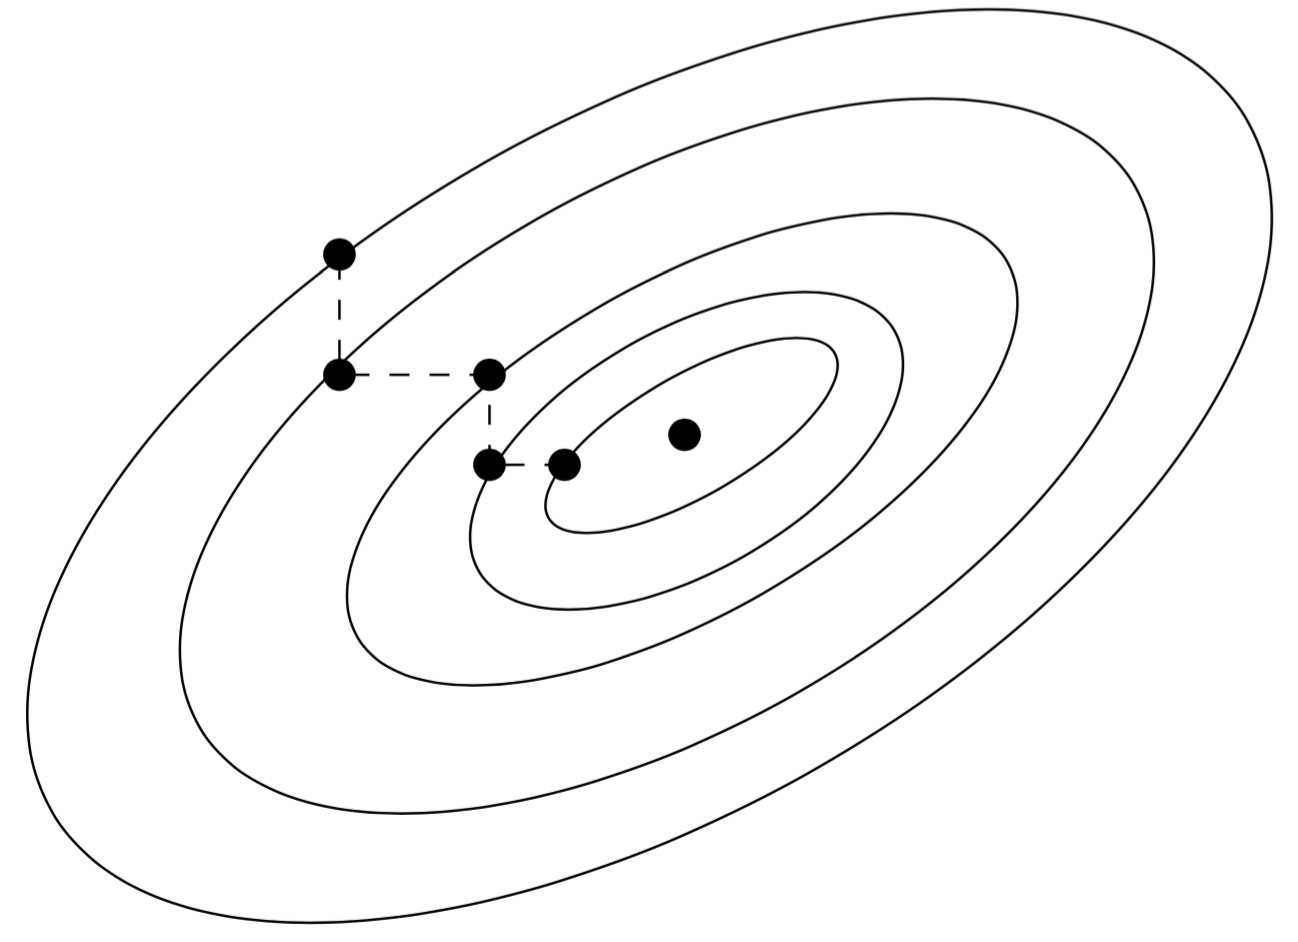
\includegraphics[scale=0.1]{pics/nc.png}
to  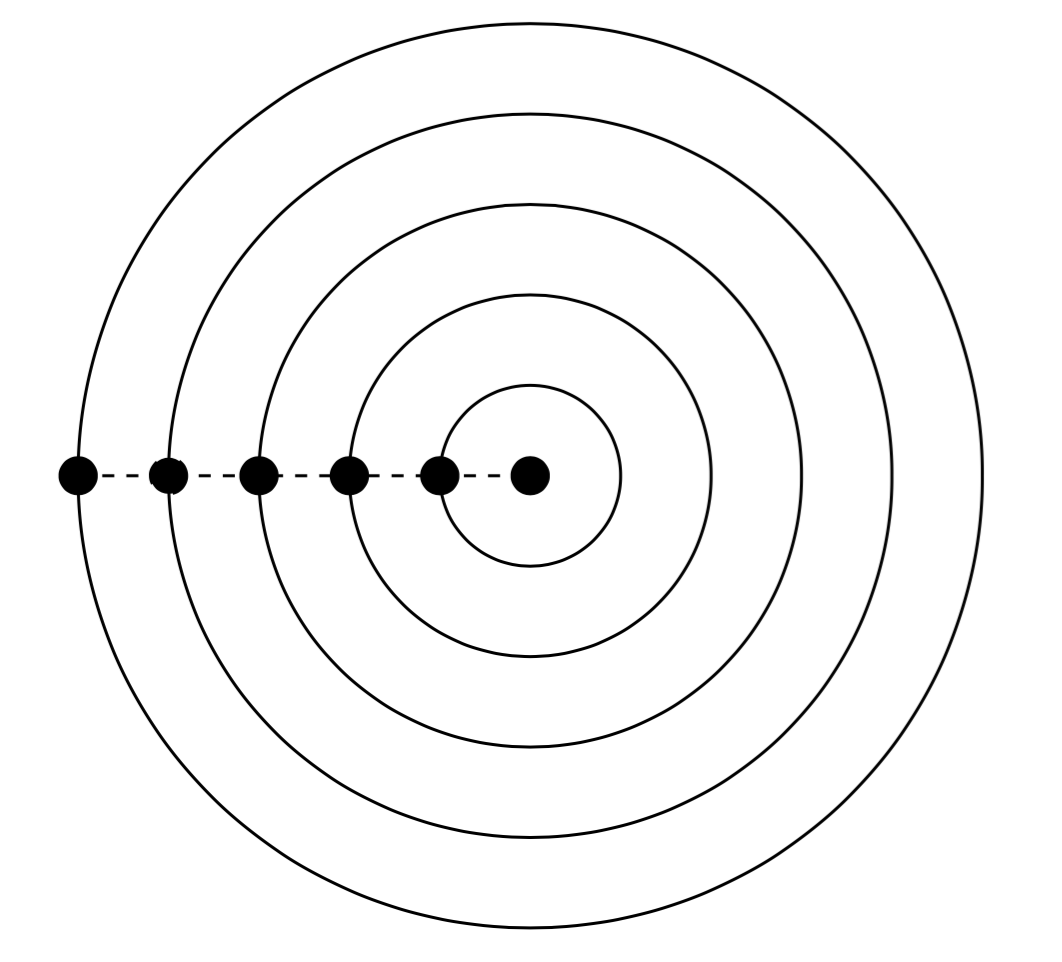
\includegraphics[scale=0.1]{pics/topview.png}

}

\only<4>{
Gradient method works well when the condition numbers are moderate,
and works poorly when the condition numbers are large.

\begin{itemize}
\item When we change the coordinates, as $\overline{x} =
  P^{\frac{1}{2}}x$, the function is moderately conditioned, the
  steepest descent method will work well.
\item $P$ should be chosen so that $f$, transformed by
  $p^{-\frac{1}{2}}$ to $\tilde{f}$, is well conditioned.
\item If approximation $\hat{H}$  of the Hessian at the optimal point
  $\hat{H}(x^*)$ were known, $P = \hat{H}$ would be a good choice, since
Hessian of at the optimum:
$$\hat{H}^{-\frac{1}{2}}\nabla^2f(x^*)\hat{H}^{\frac{1}{2}}\approx I$$
is likely to have a low condition number.
\end{itemize}
}

\only<5>{
\textbullet {\scriptsize In summary, we can say that the steepest descent method works
  well in cases where we can identify a matrix P for which the
  transformed problem has moderate condition number.}

\textbullet {\scriptsize $\cdot $ Comparison of two P norms below with the previous
  nonquadratic problem in
$R^2$, using backtracking line search parameters $\alpha = 0.1$ and
$\beta = 0.7$.
}

\vspace{-4mm}

$$P_1 = \bigl(\begin{smallmatrix}
2&0 \\ 0&8
\end{smallmatrix} \bigr) ~~and~~ P_2 = \bigl(\begin{smallmatrix}
8&0 \\ 0&2
\end{smallmatrix} \bigr)$$

\vspace{-4mm}

\begin{columns}
  \begin{column}{0.5\textwidth}
    \begin{figure}[t]
      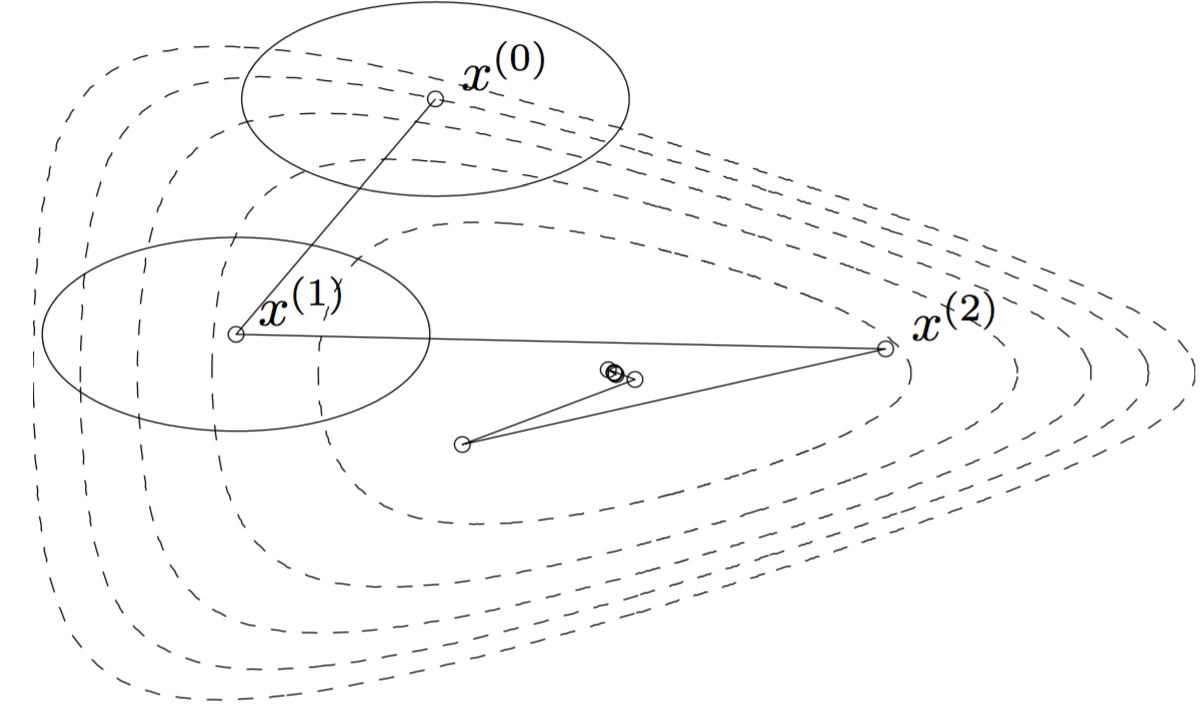
\includegraphics[scale=0.15]{pics/911.png}
      \caption{\tiny Steepest descent method, with quadratic norm
        $\norm{\cdot}_{P_1}$. The ellipses are the boundaries of the
        norm balls $\{x | \norm{x - x^{(k)}}_{P_1} \le 1\}$ at $\xk{0}
        ~and~ \xk{1}$.}
    \end{figure}
  \end{column}


  \begin{column}{0.5\textwidth}
    \begin{figure}[t]
      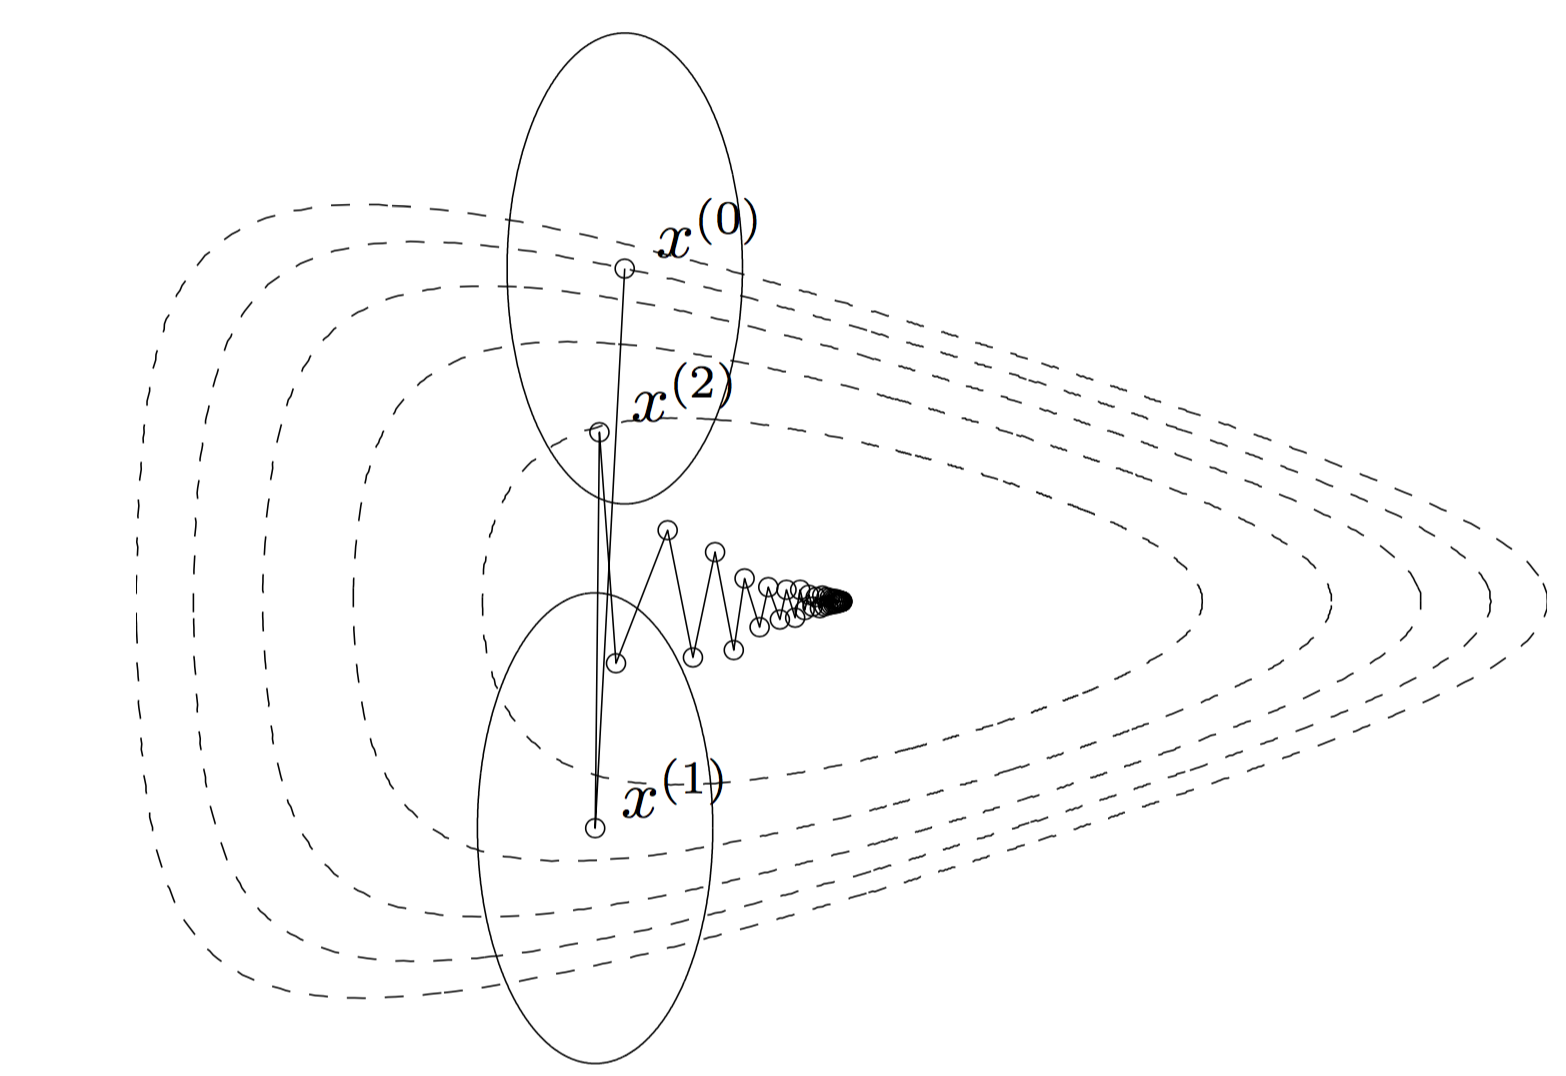
\includegraphics[scale=0.12]{pics/912.png}
      \caption{\tiny Steepest descent method, with quadratic norm
        $\norm{\cdot}_{P_2}$.}
    \end{figure}
  \end{column}
\end{columns}
}

\only<6>{
\textbullet Figure shows the error vs. iteration differences of the two norms.

\begin{columns}
  \begin{column}{0.6\textwidth}
\textbullet With the norm $\norm{\cdot}_{P_1}$, convergence is a bit more rapid
 than the gradient method, whereas with the norm $\norm{\cdot}_{P_2}$, convergence is far slower.

  \end{column}
  \begin{column}{0.5\textwidth}
    \begin{figure}[t]
      \centering
      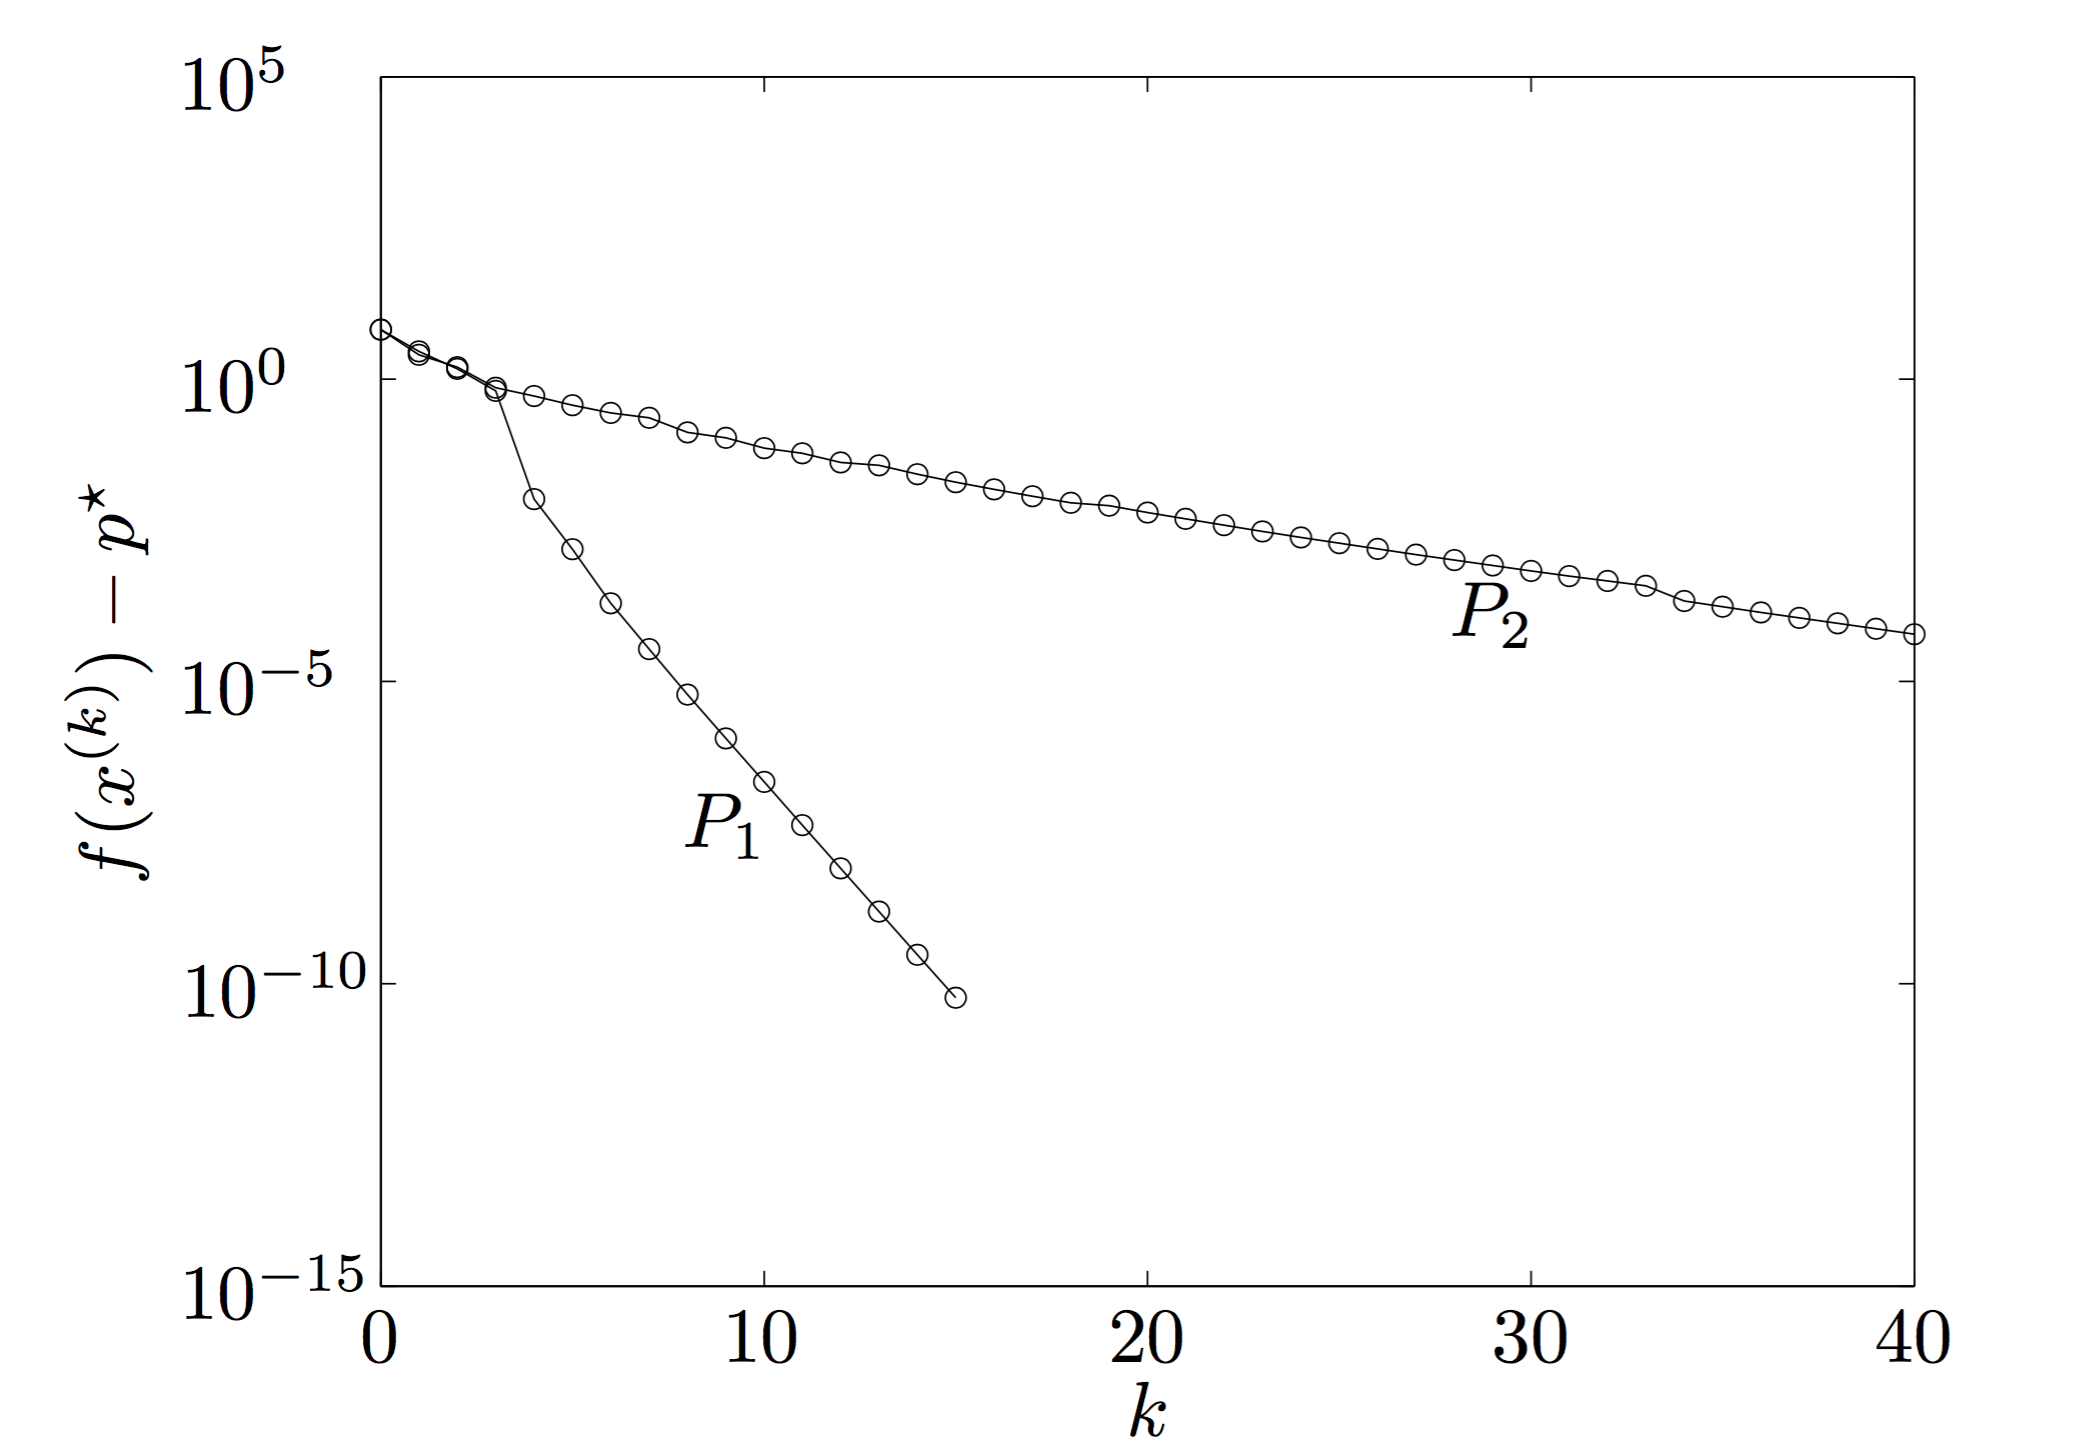
\includegraphics[scale=0.13]{pics/913.png}
      \caption{\tiny Error $f(x^*) - p^*$versus iteration k, for the
        steepest descent method with the quadratic norm
        $\norm{\cdot}_{P_1}$ and the quadratic norm
        $\norm{\cdot}_{P_2}$. Convergence is rapid for the norm $\norm{\cdot}_{P_1}$ and very slow for$\norm{\cdot}_{P_2}$.}
    \end{figure}




  \end{column}
\end{columns}

}

\only<7>{
\textbullet If we change the coordinates $\overline{x} = P_1^{\frac{1}{2}}x$,
 $\overline{x} = P_2^{\frac{1}{2}}x$ respectively we can get the following results in
transformed coordinates.


\begin{columns}
  \begin{column}{0.5\textwidth}
    \begin{figure}[bh!]
      \centering
      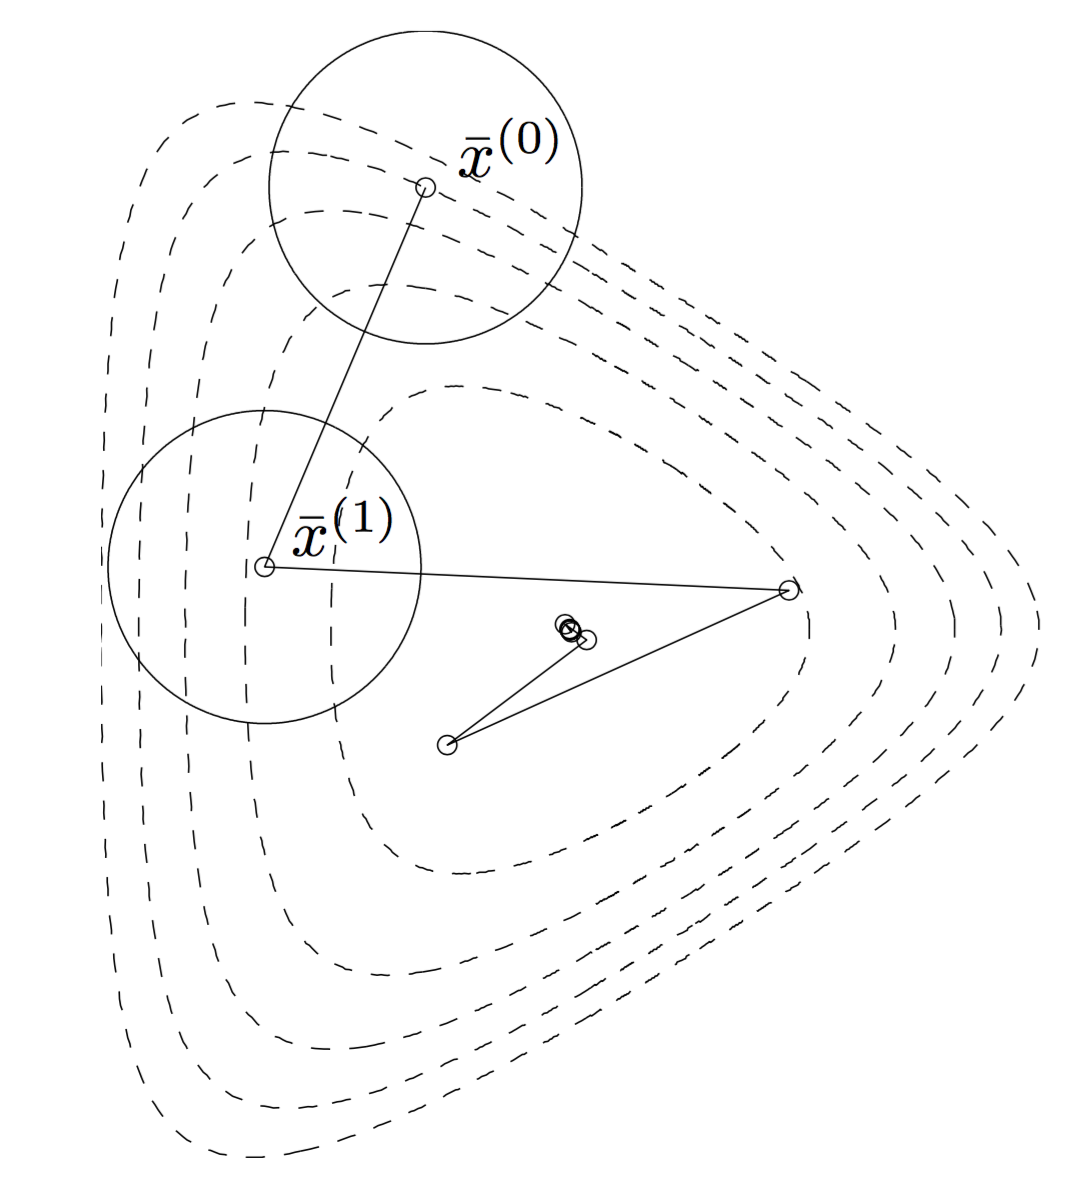
\includegraphics[scale=0.16]{pics/914.png}
      \caption{\tiny The iterates of steepest descent with norm $\norm{\cdot}_{P_1}$, after the change of coordinates. This change of coordinates reduces the condition number of the sublevel sets, and so speeds up convergence.}
    \end{figure}
  \end{column}

  \begin{column}{0.5\textwidth}
    \begin{figure}[bh!]
      \centering
      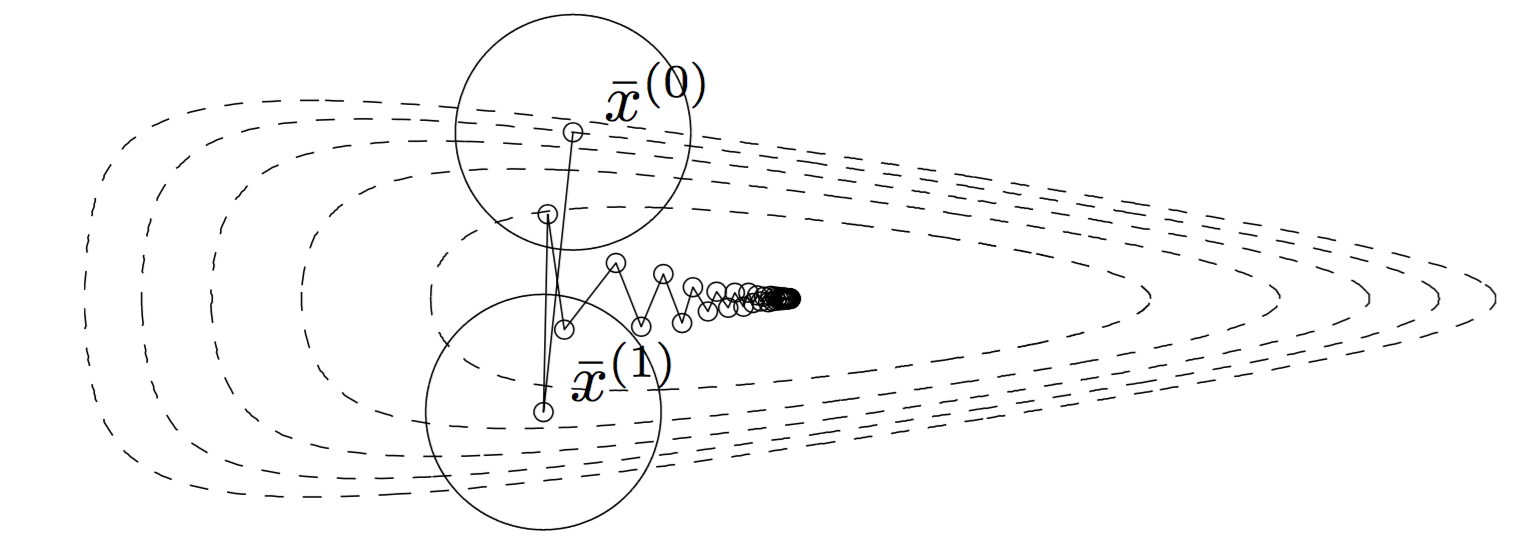
\includegraphics[scale=0.16]{pics/915.png}
      \caption{\tiny The iterates of steepest descent with norm $\norm{\cdot}_{P_1}$, after the change of coordinates. This change of coordinates increases the condition number of the sublevel sets, and so slows down convergence.}
    \end{figure}
  \end{column}
\end{columns}
}
\end{frame}
